\documentclass[twoside]{book}

% Packages required by doxygen
\usepackage{calc}
\usepackage{doxygen}
\usepackage{graphicx}
\usepackage[utf8]{inputenc}
\usepackage{makeidx}
\usepackage{multicol}
\usepackage{multirow}
\usepackage{textcomp}
\usepackage[table]{xcolor}

% Font selection
\usepackage[T1]{fontenc}
\usepackage{mathptmx}
\usepackage[scaled=.90]{helvet}
\usepackage{courier}
\usepackage{amssymb}
\usepackage{sectsty}
\renewcommand{\familydefault}{\sfdefault}
\allsectionsfont{%
  \fontseries{bc}\selectfont%
  \color{darkgray}%
}
\renewcommand{\DoxyLabelFont}{%
  \fontseries{bc}\selectfont%
  \color{darkgray}%
}

% Page & text layout
\usepackage{geometry}
\geometry{%
  a4paper,%
  top=2.5cm,%
  bottom=2.5cm,%
  left=2.5cm,%
  right=2.5cm%
}
\tolerance=750
\hfuzz=15pt
\hbadness=750
\setlength{\emergencystretch}{15pt}
\setlength{\parindent}{0cm}
\setlength{\parskip}{0.2cm}
\makeatletter
\renewcommand{\paragraph}{%
  \@startsection{paragraph}{4}{0ex}{-1.0ex}{1.0ex}{%
    \normalfont\normalsize\bfseries\SS@parafont%
  }%
}
\renewcommand{\subparagraph}{%
  \@startsection{subparagraph}{5}{0ex}{-1.0ex}{1.0ex}{%
    \normalfont\normalsize\bfseries\SS@subparafont%
  }%
}
\makeatother

% Headers & footers
\usepackage{fancyhdr}
\pagestyle{fancyplain}
\fancyhead[LE]{\fancyplain{}{\bfseries\thepage}}
\fancyhead[CE]{\fancyplain{}{}}
\fancyhead[RE]{\fancyplain{}{\bfseries\leftmark}}
\fancyhead[LO]{\fancyplain{}{\bfseries\rightmark}}
\fancyhead[CO]{\fancyplain{}{}}
\fancyhead[RO]{\fancyplain{}{\bfseries\thepage}}
\fancyfoot[LE]{\fancyplain{}{}}
\fancyfoot[CE]{\fancyplain{}{}}
\fancyfoot[RE]{\fancyplain{}{\bfseries\scriptsize Generated on Mon Jan 20 2014 17\-:20\-:27 for Meguno\-Link Pro Arduino Library by Doxygen }}
\fancyfoot[LO]{\fancyplain{}{\bfseries\scriptsize Generated on Mon Jan 20 2014 17\-:20\-:27 for Meguno\-Link Pro Arduino Library by Doxygen }}
\fancyfoot[CO]{\fancyplain{}{}}
\fancyfoot[RO]{\fancyplain{}{}}
\renewcommand{\footrulewidth}{0.4pt}
\renewcommand{\chaptermark}[1]{%
  \markboth{#1}{}%
}
\renewcommand{\sectionmark}[1]{%
  \markright{\thesection\ #1}%
}

% Indices & bibliography
\usepackage{natbib}
\usepackage[titles]{tocloft}
\setcounter{tocdepth}{3}
\setcounter{secnumdepth}{5}
\makeindex

% Hyperlinks (required, but should be loaded last)
\usepackage{ifpdf}
\ifpdf
  \usepackage[pdftex,pagebackref=true]{hyperref}
\else
  \usepackage[ps2pdf,pagebackref=true]{hyperref}
\fi
\hypersetup{%
  colorlinks=true,%
  linkcolor=blue,%
  citecolor=blue,%
  unicode%
}

% Custom commands
\newcommand{\clearemptydoublepage}{%
  \newpage{\pagestyle{empty}\cleardoublepage}%
}


%===== C O N T E N T S =====

\begin{document}

% Titlepage & ToC
\hypersetup{pageanchor=false}
\pagenumbering{roman}
\begin{titlepage}
\vspace*{7cm}
\begin{center}%
{\Large Meguno\-Link Pro Arduino Library }\\
\vspace*{1cm}
{\large Generated by Doxygen 1.8.6}\\
\vspace*{0.5cm}
{\small Mon Jan 20 2014 17:20:27}\\
\end{center}
\end{titlepage}
\clearemptydoublepage
\tableofcontents
\clearemptydoublepage
\pagenumbering{arabic}
\hypersetup{pageanchor=true}

%--- Begin generated contents ---
\chapter{M\-L\-P}
\label{md___dropbox__arduino_development__git_hub__m_l_p__r_e_a_d_m_e}
\hypertarget{md___dropbox__arduino_development__git_hub__m_l_p__r_e_a_d_m_e}{}
An Arduino library for sending Meguno\-Link Pro packets to the various visualisers. Currently supports sending data to\-:
\begin{DoxyItemize}
\item \href{http://www.megunolink.com/documentation/plotting/}{\tt X\-Y-\/\-Plots}
\item \href{http://www.megunolink.com/documentation/plotting/}{\tt Time plots}
\item \href{http://www.megunolink.com/documentation/table/}{\tt Tables}
\item \href{http://www.megunolink.com/documentation/mapping/}{\tt Maps}
\item \href{http://www.megunolink.com/documentation/interface-panel/}{\tt Interface panel}
\item \href{http://www.megunolink.com/documentation/monitoring-data/}{\tt Message stream}
\end{DoxyItemize}

Visit www.\-Meguno\-Link.\-com to download a free trial of \href{http://www.MegunoLink.com}{\tt Meguno\-Link Pro}. 
\chapter{Hierarchical Index}
\section{Class Hierarchy}
This inheritance list is sorted roughly, but not completely, alphabetically\-:\begin{DoxyCompactList}
\item \contentsline{section}{Meguno\-Link\-Protocol}{\pageref{class_meguno_link_protocol}}{}
\begin{DoxyCompactList}
\item \contentsline{section}{Interface\-Panel}{\pageref{class_interface_panel}}{}
\item \contentsline{section}{Map}{\pageref{class_map}}{}
\item \contentsline{section}{Message}{\pageref{class_message}}{}
\item \contentsline{section}{Plot}{\pageref{class_plot}}{}
\begin{DoxyCompactList}
\item \contentsline{section}{Time\-Plot}{\pageref{class_time_plot}}{}
\item \contentsline{section}{X\-Y\-Plot}{\pageref{class_x_y_plot}}{}
\end{DoxyCompactList}
\item \contentsline{section}{Table}{\pageref{class_table}}{}
\end{DoxyCompactList}
\end{DoxyCompactList}

\chapter{Class Index}
\section{Class List}
Here are the classes, structs, unions and interfaces with brief descriptions\-:\begin{DoxyCompactList}
\item\contentsline{section}{\hyperlink{class_interface_panel}{Interface\-Panel} }{\pageref{class_interface_panel}}{}
\item\contentsline{section}{\hyperlink{class_map}{Map} }{\pageref{class_map}}{}
\item\contentsline{section}{\hyperlink{class_meguno_link_protocol}{Meguno\-Link\-Protocol} }{\pageref{class_meguno_link_protocol}}{}
\item\contentsline{section}{\hyperlink{class_message}{Message} }{\pageref{class_message}}{}
\item\contentsline{section}{\hyperlink{class_plot}{Plot} }{\pageref{class_plot}}{}
\item\contentsline{section}{\hyperlink{class_table}{Table} }{\pageref{class_table}}{}
\item\contentsline{section}{\hyperlink{class_time_plot}{Time\-Plot} }{\pageref{class_time_plot}}{}
\item\contentsline{section}{\hyperlink{class_x_y_plot}{X\-Y\-Plot} }{\pageref{class_x_y_plot}}{}
\end{DoxyCompactList}

\chapter{File Index}
\section{File List}
Here is a list of all files with brief descriptions\-:\begin{DoxyCompactList}
\item\contentsline{section}{/\-Dropbox/\-Arduino\-Development/\-Git\-Hub/\-M\-L\-P/\hyperlink{_meguno_link_8h}{Meguno\-Link.\-h} }{\pageref{_meguno_link_8h}}{}
\item\contentsline{section}{/\-Dropbox/\-Arduino\-Development/\-Git\-Hub/\-M\-L\-P/utility/\hyperlink{_interface_panel_8cpp}{Interface\-Panel.\-cpp} }{\pageref{_interface_panel_8cpp}}{}
\item\contentsline{section}{/\-Dropbox/\-Arduino\-Development/\-Git\-Hub/\-M\-L\-P/utility/\hyperlink{_interface_panel_8h}{Interface\-Panel.\-h} }{\pageref{_interface_panel_8h}}{}
\item\contentsline{section}{/\-Dropbox/\-Arduino\-Development/\-Git\-Hub/\-M\-L\-P/utility/\hyperlink{_map_8cpp}{Map.\-cpp} }{\pageref{_map_8cpp}}{}
\item\contentsline{section}{/\-Dropbox/\-Arduino\-Development/\-Git\-Hub/\-M\-L\-P/utility/\hyperlink{_map_8h}{Map.\-h} }{\pageref{_map_8h}}{}
\item\contentsline{section}{/\-Dropbox/\-Arduino\-Development/\-Git\-Hub/\-M\-L\-P/utility/\hyperlink{_meguno_link_protocol_8cpp}{Meguno\-Link\-Protocol.\-cpp} }{\pageref{_meguno_link_protocol_8cpp}}{}
\item\contentsline{section}{/\-Dropbox/\-Arduino\-Development/\-Git\-Hub/\-M\-L\-P/utility/\hyperlink{_meguno_link_protocol_8h}{Meguno\-Link\-Protocol.\-h} }{\pageref{_meguno_link_protocol_8h}}{}
\item\contentsline{section}{/\-Dropbox/\-Arduino\-Development/\-Git\-Hub/\-M\-L\-P/utility/\hyperlink{_message_8cpp}{Message.\-cpp} }{\pageref{_message_8cpp}}{}
\item\contentsline{section}{/\-Dropbox/\-Arduino\-Development/\-Git\-Hub/\-M\-L\-P/utility/\hyperlink{_message_8h}{Message.\-h} }{\pageref{_message_8h}}{}
\item\contentsline{section}{/\-Dropbox/\-Arduino\-Development/\-Git\-Hub/\-M\-L\-P/utility/\hyperlink{_plot_8cpp}{Plot.\-cpp} }{\pageref{_plot_8cpp}}{}
\item\contentsline{section}{/\-Dropbox/\-Arduino\-Development/\-Git\-Hub/\-M\-L\-P/utility/\hyperlink{_plot_8h}{Plot.\-h} }{\pageref{_plot_8h}}{}
\item\contentsline{section}{/\-Dropbox/\-Arduino\-Development/\-Git\-Hub/\-M\-L\-P/utility/\hyperlink{_table_8cpp}{Table.\-cpp} }{\pageref{_table_8cpp}}{}
\item\contentsline{section}{/\-Dropbox/\-Arduino\-Development/\-Git\-Hub/\-M\-L\-P/utility/\hyperlink{_table_8h}{Table.\-h} }{\pageref{_table_8h}}{}
\item\contentsline{section}{/\-Dropbox/\-Arduino\-Development/\-Git\-Hub/\-M\-L\-P/utility/\hyperlink{_time_plot_8cpp}{Time\-Plot.\-cpp} }{\pageref{_time_plot_8cpp}}{}
\item\contentsline{section}{/\-Dropbox/\-Arduino\-Development/\-Git\-Hub/\-M\-L\-P/utility/\hyperlink{_time_plot_8h}{Time\-Plot.\-h} }{\pageref{_time_plot_8h}}{}
\item\contentsline{section}{/\-Dropbox/\-Arduino\-Development/\-Git\-Hub/\-M\-L\-P/utility/\hyperlink{_x_y_plot_8cpp}{X\-Y\-Plot.\-cpp} }{\pageref{_x_y_plot_8cpp}}{}
\item\contentsline{section}{/\-Dropbox/\-Arduino\-Development/\-Git\-Hub/\-M\-L\-P/utility/\hyperlink{_x_y_plot_8h}{X\-Y\-Plot.\-h} }{\pageref{_x_y_plot_8h}}{}
\end{DoxyCompactList}

\chapter{Class Documentation}
\hypertarget{class_interface_panel}{\section{Interface\-Panel Class Reference}
\label{class_interface_panel}\index{Interface\-Panel@{Interface\-Panel}}
}


{\ttfamily \#include $<$Interface\-Panel.\-h$>$}

Inheritance diagram for Interface\-Panel\-:\begin{figure}[H]
\begin{center}
\leavevmode
\includegraphics[height=2.000000cm]{class_interface_panel}
\end{center}
\end{figure}
\subsection*{Public Member Functions}
\begin{DoxyCompactItemize}
\item 
\hyperlink{class_interface_panel_ac7d304958b61155401f0ebbc2fc427a7}{Interface\-Panel} (const char $\ast$channel\-Name=N\-U\-L\-L)
\item 
\hyperlink{class_interface_panel_a4a7e5b5fa82501da446edff5e8a91f4b}{Interface\-Panel} (const \-\_\-\-\_\-\-Flash\-String\-Helper $\ast$channel\-Name)
\item 
void \hyperlink{class_interface_panel_a3bac571aa848d37e1fd23d9551ceacf9}{Set\-Text} (const char $\ast$Control\-Name, const char $\ast$Value)
\item 
void \hyperlink{class_interface_panel_acd10e08c8c9c4e01d622b9d6ed820ca2}{Set\-Text} (const \-\_\-\-\_\-\-Flash\-String\-Helper $\ast$Control\-Name, const char $\ast$Value)
\item 
void \hyperlink{class_interface_panel_accfbc36dbac07f787057207243733284}{Set\-Text} (const \-\_\-\-\_\-\-Flash\-String\-Helper $\ast$Control\-Name, const \-\_\-\-\_\-\-Flash\-String\-Helper $\ast$Value)
\item 
void \hyperlink{class_interface_panel_a8c318680d9a47f4362ce9f24c5cd883d}{Set\-Progress} (const char $\ast$Control\-Name, int n\-Value)
\item 
void \hyperlink{class_interface_panel_a47f11df228897dccb36e50258054d104}{Set\-Progress} (const \-\_\-\-\_\-\-Flash\-String\-Helper $\ast$Control\-Name, int n\-Value)
\item 
void \hyperlink{class_interface_panel_adccffdc7239c79e8afd8cf9be768fdef}{Set\-Number} (const char $\ast$Control\-Name, int n\-Value)
\item 
void \hyperlink{class_interface_panel_a4973b1694aa8ab390d3199ba28939491}{Set\-Number} (const \-\_\-\-\_\-\-Flash\-String\-Helper $\ast$Control\-Name, int n\-Value)
\item 
void \hyperlink{class_interface_panel_a4cc8cf346c34a2713253c96d295361d3}{Set\-Check} (const char $\ast$Control\-Name, bool b\-Checked=true)
\item 
void \hyperlink{class_interface_panel_aff2ae872c64b2271e60d245b2a910962}{Set\-Check} (const \-\_\-\-\_\-\-Flash\-String\-Helper $\ast$Control\-Name, bool b\-Checked=true)
\item 
void \hyperlink{class_interface_panel_a6dc489a049643e7c8eb93122a8bb7917}{Clear\-Check} (const char $\ast$Control\-Name)
\item 
void \hyperlink{class_interface_panel_a7908e97410a75e652cb2d860ad99dfe1}{Clear\-Check} (const \-\_\-\-\_\-\-Flash\-String\-Helper $\ast$Control\-Name)
\end{DoxyCompactItemize}
\subsection*{Protected Member Functions}
\begin{DoxyCompactItemize}
\item 
void \hyperlink{class_interface_panel_af56161722f9f4bcfb50c1ebae9bea28b}{Send\-Control\-Header} (const char $\ast$Control\-Name, const \-\_\-\-\_\-\-Flash\-String\-Helper $\ast$Property\-Name)
\item 
void \hyperlink{class_interface_panel_a64bf7ca35205c00547225c53e930f5b8}{Send\-Control\-Header} (const \-\_\-\-\_\-\-Flash\-String\-Helper $\ast$Control\-Name, const \-\_\-\-\_\-\-Flash\-String\-Helper $\ast$Property\-Name)
\end{DoxyCompactItemize}


\subsection{Constructor \& Destructor Documentation}
\hypertarget{class_interface_panel_ac7d304958b61155401f0ebbc2fc427a7}{\index{Interface\-Panel@{Interface\-Panel}!Interface\-Panel@{Interface\-Panel}}
\index{Interface\-Panel@{Interface\-Panel}!InterfacePanel@{Interface\-Panel}}
\subsubsection[{Interface\-Panel}]{\setlength{\rightskip}{0pt plus 5cm}Interface\-Panel\-::\-Interface\-Panel (
\begin{DoxyParamCaption}
\item[{const char $\ast$}]{channel\-Name = {\ttfamily NULL}}
\end{DoxyParamCaption}
)}}\label{class_interface_panel_ac7d304958b61155401f0ebbc2fc427a7}
\hypertarget{class_interface_panel_a4a7e5b5fa82501da446edff5e8a91f4b}{\index{Interface\-Panel@{Interface\-Panel}!Interface\-Panel@{Interface\-Panel}}
\index{Interface\-Panel@{Interface\-Panel}!InterfacePanel@{Interface\-Panel}}
\subsubsection[{Interface\-Panel}]{\setlength{\rightskip}{0pt plus 5cm}Interface\-Panel\-::\-Interface\-Panel (
\begin{DoxyParamCaption}
\item[{const \-\_\-\-\_\-\-Flash\-String\-Helper $\ast$}]{channel\-Name}
\end{DoxyParamCaption}
)}}\label{class_interface_panel_a4a7e5b5fa82501da446edff5e8a91f4b}


\subsection{Member Function Documentation}
\hypertarget{class_interface_panel_a6dc489a049643e7c8eb93122a8bb7917}{\index{Interface\-Panel@{Interface\-Panel}!Clear\-Check@{Clear\-Check}}
\index{Clear\-Check@{Clear\-Check}!InterfacePanel@{Interface\-Panel}}
\subsubsection[{Clear\-Check}]{\setlength{\rightskip}{0pt plus 5cm}void Interface\-Panel\-::\-Clear\-Check (
\begin{DoxyParamCaption}
\item[{const char $\ast$}]{Control\-Name}
\end{DoxyParamCaption}
)}}\label{class_interface_panel_a6dc489a049643e7c8eb93122a8bb7917}
\hypertarget{class_interface_panel_a7908e97410a75e652cb2d860ad99dfe1}{\index{Interface\-Panel@{Interface\-Panel}!Clear\-Check@{Clear\-Check}}
\index{Clear\-Check@{Clear\-Check}!InterfacePanel@{Interface\-Panel}}
\subsubsection[{Clear\-Check}]{\setlength{\rightskip}{0pt plus 5cm}void Interface\-Panel\-::\-Clear\-Check (
\begin{DoxyParamCaption}
\item[{const \-\_\-\-\_\-\-Flash\-String\-Helper $\ast$}]{Control\-Name}
\end{DoxyParamCaption}
)}}\label{class_interface_panel_a7908e97410a75e652cb2d860ad99dfe1}
\hypertarget{class_interface_panel_af56161722f9f4bcfb50c1ebae9bea28b}{\index{Interface\-Panel@{Interface\-Panel}!Send\-Control\-Header@{Send\-Control\-Header}}
\index{Send\-Control\-Header@{Send\-Control\-Header}!InterfacePanel@{Interface\-Panel}}
\subsubsection[{Send\-Control\-Header}]{\setlength{\rightskip}{0pt plus 5cm}void Interface\-Panel\-::\-Send\-Control\-Header (
\begin{DoxyParamCaption}
\item[{const char $\ast$}]{Control\-Name, }
\item[{const \-\_\-\-\_\-\-Flash\-String\-Helper $\ast$}]{Property\-Name}
\end{DoxyParamCaption}
)\hspace{0.3cm}{\ttfamily [protected]}}}\label{class_interface_panel_af56161722f9f4bcfb50c1ebae9bea28b}
\hypertarget{class_interface_panel_a64bf7ca35205c00547225c53e930f5b8}{\index{Interface\-Panel@{Interface\-Panel}!Send\-Control\-Header@{Send\-Control\-Header}}
\index{Send\-Control\-Header@{Send\-Control\-Header}!InterfacePanel@{Interface\-Panel}}
\subsubsection[{Send\-Control\-Header}]{\setlength{\rightskip}{0pt plus 5cm}void Interface\-Panel\-::\-Send\-Control\-Header (
\begin{DoxyParamCaption}
\item[{const \-\_\-\-\_\-\-Flash\-String\-Helper $\ast$}]{Control\-Name, }
\item[{const \-\_\-\-\_\-\-Flash\-String\-Helper $\ast$}]{Property\-Name}
\end{DoxyParamCaption}
)\hspace{0.3cm}{\ttfamily [protected]}}}\label{class_interface_panel_a64bf7ca35205c00547225c53e930f5b8}
\hypertarget{class_interface_panel_a4cc8cf346c34a2713253c96d295361d3}{\index{Interface\-Panel@{Interface\-Panel}!Set\-Check@{Set\-Check}}
\index{Set\-Check@{Set\-Check}!InterfacePanel@{Interface\-Panel}}
\subsubsection[{Set\-Check}]{\setlength{\rightskip}{0pt plus 5cm}void Interface\-Panel\-::\-Set\-Check (
\begin{DoxyParamCaption}
\item[{const char $\ast$}]{Control\-Name, }
\item[{bool}]{b\-Checked = {\ttfamily true}}
\end{DoxyParamCaption}
)}}\label{class_interface_panel_a4cc8cf346c34a2713253c96d295361d3}
\hypertarget{class_interface_panel_aff2ae872c64b2271e60d245b2a910962}{\index{Interface\-Panel@{Interface\-Panel}!Set\-Check@{Set\-Check}}
\index{Set\-Check@{Set\-Check}!InterfacePanel@{Interface\-Panel}}
\subsubsection[{Set\-Check}]{\setlength{\rightskip}{0pt plus 5cm}void Interface\-Panel\-::\-Set\-Check (
\begin{DoxyParamCaption}
\item[{const \-\_\-\-\_\-\-Flash\-String\-Helper $\ast$}]{Control\-Name, }
\item[{bool}]{b\-Checked = {\ttfamily true}}
\end{DoxyParamCaption}
)}}\label{class_interface_panel_aff2ae872c64b2271e60d245b2a910962}
\hypertarget{class_interface_panel_adccffdc7239c79e8afd8cf9be768fdef}{\index{Interface\-Panel@{Interface\-Panel}!Set\-Number@{Set\-Number}}
\index{Set\-Number@{Set\-Number}!InterfacePanel@{Interface\-Panel}}
\subsubsection[{Set\-Number}]{\setlength{\rightskip}{0pt plus 5cm}void Interface\-Panel\-::\-Set\-Number (
\begin{DoxyParamCaption}
\item[{const char $\ast$}]{Control\-Name, }
\item[{int}]{n\-Value}
\end{DoxyParamCaption}
)}}\label{class_interface_panel_adccffdc7239c79e8afd8cf9be768fdef}
\hypertarget{class_interface_panel_a4973b1694aa8ab390d3199ba28939491}{\index{Interface\-Panel@{Interface\-Panel}!Set\-Number@{Set\-Number}}
\index{Set\-Number@{Set\-Number}!InterfacePanel@{Interface\-Panel}}
\subsubsection[{Set\-Number}]{\setlength{\rightskip}{0pt plus 5cm}void Interface\-Panel\-::\-Set\-Number (
\begin{DoxyParamCaption}
\item[{const \-\_\-\-\_\-\-Flash\-String\-Helper $\ast$}]{Control\-Name, }
\item[{int}]{n\-Value}
\end{DoxyParamCaption}
)}}\label{class_interface_panel_a4973b1694aa8ab390d3199ba28939491}
\hypertarget{class_interface_panel_a8c318680d9a47f4362ce9f24c5cd883d}{\index{Interface\-Panel@{Interface\-Panel}!Set\-Progress@{Set\-Progress}}
\index{Set\-Progress@{Set\-Progress}!InterfacePanel@{Interface\-Panel}}
\subsubsection[{Set\-Progress}]{\setlength{\rightskip}{0pt plus 5cm}void Interface\-Panel\-::\-Set\-Progress (
\begin{DoxyParamCaption}
\item[{const char $\ast$}]{Control\-Name, }
\item[{int}]{n\-Value}
\end{DoxyParamCaption}
)}}\label{class_interface_panel_a8c318680d9a47f4362ce9f24c5cd883d}
\hypertarget{class_interface_panel_a47f11df228897dccb36e50258054d104}{\index{Interface\-Panel@{Interface\-Panel}!Set\-Progress@{Set\-Progress}}
\index{Set\-Progress@{Set\-Progress}!InterfacePanel@{Interface\-Panel}}
\subsubsection[{Set\-Progress}]{\setlength{\rightskip}{0pt plus 5cm}void Interface\-Panel\-::\-Set\-Progress (
\begin{DoxyParamCaption}
\item[{const \-\_\-\-\_\-\-Flash\-String\-Helper $\ast$}]{Control\-Name, }
\item[{int}]{n\-Value}
\end{DoxyParamCaption}
)}}\label{class_interface_panel_a47f11df228897dccb36e50258054d104}
\hypertarget{class_interface_panel_a3bac571aa848d37e1fd23d9551ceacf9}{\index{Interface\-Panel@{Interface\-Panel}!Set\-Text@{Set\-Text}}
\index{Set\-Text@{Set\-Text}!InterfacePanel@{Interface\-Panel}}
\subsubsection[{Set\-Text}]{\setlength{\rightskip}{0pt plus 5cm}void Interface\-Panel\-::\-Set\-Text (
\begin{DoxyParamCaption}
\item[{const char $\ast$}]{Control\-Name, }
\item[{const char $\ast$}]{Value}
\end{DoxyParamCaption}
)}}\label{class_interface_panel_a3bac571aa848d37e1fd23d9551ceacf9}
\hypertarget{class_interface_panel_acd10e08c8c9c4e01d622b9d6ed820ca2}{\index{Interface\-Panel@{Interface\-Panel}!Set\-Text@{Set\-Text}}
\index{Set\-Text@{Set\-Text}!InterfacePanel@{Interface\-Panel}}
\subsubsection[{Set\-Text}]{\setlength{\rightskip}{0pt plus 5cm}void Interface\-Panel\-::\-Set\-Text (
\begin{DoxyParamCaption}
\item[{const \-\_\-\-\_\-\-Flash\-String\-Helper $\ast$}]{Control\-Name, }
\item[{const char $\ast$}]{Value}
\end{DoxyParamCaption}
)}}\label{class_interface_panel_acd10e08c8c9c4e01d622b9d6ed820ca2}
\hypertarget{class_interface_panel_accfbc36dbac07f787057207243733284}{\index{Interface\-Panel@{Interface\-Panel}!Set\-Text@{Set\-Text}}
\index{Set\-Text@{Set\-Text}!InterfacePanel@{Interface\-Panel}}
\subsubsection[{Set\-Text}]{\setlength{\rightskip}{0pt plus 5cm}void Interface\-Panel\-::\-Set\-Text (
\begin{DoxyParamCaption}
\item[{const \-\_\-\-\_\-\-Flash\-String\-Helper $\ast$}]{Control\-Name, }
\item[{const \-\_\-\-\_\-\-Flash\-String\-Helper $\ast$}]{Value}
\end{DoxyParamCaption}
)}}\label{class_interface_panel_accfbc36dbac07f787057207243733284}


The documentation for this class was generated from the following files\-:\begin{DoxyCompactItemize}
\item 
/\-Dropbox/\-Arduino\-Development/\-Git\-Hub/\-M\-L\-P/utility/\hyperlink{_interface_panel_8h}{Interface\-Panel.\-h}\item 
/\-Dropbox/\-Arduino\-Development/\-Git\-Hub/\-M\-L\-P/utility/\hyperlink{_interface_panel_8cpp}{Interface\-Panel.\-cpp}\end{DoxyCompactItemize}

\hypertarget{class_map}{\section{Map Class Reference}
\label{class_map}\index{Map@{Map}}
}


{\ttfamily \#include $<$Map.\-h$>$}

Inheritance diagram for Map\-:\begin{figure}[H]
\begin{center}
\leavevmode
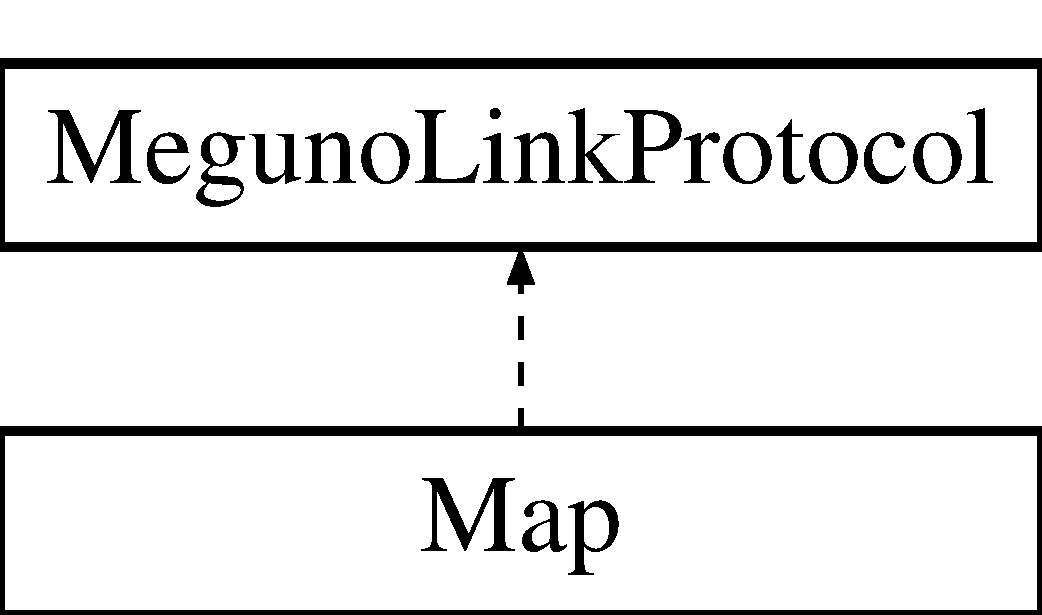
\includegraphics[height=2.000000cm]{class_map}
\end{center}
\end{figure}
\subsection*{Public Member Functions}
\begin{DoxyCompactItemize}
\item 
\hyperlink{class_map_a0f5ad0fd4563497b4214038cbca8b582}{Map} ()
\item 
void \hyperlink{class_map_a5aedb8d21392bb88ff901c686c5ac1b5}{Send\-Data} (const char $\ast$Placename, const char $\ast$Latitude, const char $\ast$Longitude)
\item 
void \hyperlink{class_map_a5c5221e4c694172f06a9a63092130f19}{Send\-Data} (const \-\_\-\-\_\-\-Flash\-String\-Helper $\ast$Placename, const char $\ast$Latitude, const char $\ast$Longitude)
\item 
void \hyperlink{class_map_aa6d89c6c2f568bfc563ab67720996249}{Send\-Data} (const char $\ast$Placename, float Latitude, float Longitude)
\item 
void \hyperlink{class_map_a6f2175798dcb22972fea69e2224842e6}{Send\-Data} (const \-\_\-\-\_\-\-Flash\-String\-Helper $\ast$Placename, float Latitude, float Longitude)
\end{DoxyCompactItemize}
\subsection*{Additional Inherited Members}


\subsection{Constructor \& Destructor Documentation}
\hypertarget{class_map_a0f5ad0fd4563497b4214038cbca8b582}{\index{Map@{Map}!Map@{Map}}
\index{Map@{Map}!Map@{Map}}
\subsubsection[{Map}]{\setlength{\rightskip}{0pt plus 5cm}Map\-::\-Map (
\begin{DoxyParamCaption}
{}
\end{DoxyParamCaption}
)}}\label{class_map_a0f5ad0fd4563497b4214038cbca8b582}


\subsection{Member Function Documentation}
\hypertarget{class_map_a5aedb8d21392bb88ff901c686c5ac1b5}{\index{Map@{Map}!Send\-Data@{Send\-Data}}
\index{Send\-Data@{Send\-Data}!Map@{Map}}
\subsubsection[{Send\-Data}]{\setlength{\rightskip}{0pt plus 5cm}void Map\-::\-Send\-Data (
\begin{DoxyParamCaption}
\item[{const char $\ast$}]{Placename, }
\item[{const char $\ast$}]{Latitude, }
\item[{const char $\ast$}]{Longitude}
\end{DoxyParamCaption}
)}}\label{class_map_a5aedb8d21392bb88ff901c686c5ac1b5}
\hypertarget{class_map_a5c5221e4c694172f06a9a63092130f19}{\index{Map@{Map}!Send\-Data@{Send\-Data}}
\index{Send\-Data@{Send\-Data}!Map@{Map}}
\subsubsection[{Send\-Data}]{\setlength{\rightskip}{0pt plus 5cm}void Map\-::\-Send\-Data (
\begin{DoxyParamCaption}
\item[{const \-\_\-\-\_\-\-Flash\-String\-Helper $\ast$}]{Placename, }
\item[{const char $\ast$}]{Latitude, }
\item[{const char $\ast$}]{Longitude}
\end{DoxyParamCaption}
)}}\label{class_map_a5c5221e4c694172f06a9a63092130f19}
\hypertarget{class_map_aa6d89c6c2f568bfc563ab67720996249}{\index{Map@{Map}!Send\-Data@{Send\-Data}}
\index{Send\-Data@{Send\-Data}!Map@{Map}}
\subsubsection[{Send\-Data}]{\setlength{\rightskip}{0pt plus 5cm}void Map\-::\-Send\-Data (
\begin{DoxyParamCaption}
\item[{const char $\ast$}]{Placename, }
\item[{float}]{Latitude, }
\item[{float}]{Longitude}
\end{DoxyParamCaption}
)}}\label{class_map_aa6d89c6c2f568bfc563ab67720996249}
\hypertarget{class_map_a6f2175798dcb22972fea69e2224842e6}{\index{Map@{Map}!Send\-Data@{Send\-Data}}
\index{Send\-Data@{Send\-Data}!Map@{Map}}
\subsubsection[{Send\-Data}]{\setlength{\rightskip}{0pt plus 5cm}void Map\-::\-Send\-Data (
\begin{DoxyParamCaption}
\item[{const \-\_\-\-\_\-\-Flash\-String\-Helper $\ast$}]{Placename, }
\item[{float}]{Latitude, }
\item[{float}]{Longitude}
\end{DoxyParamCaption}
)}}\label{class_map_a6f2175798dcb22972fea69e2224842e6}


The documentation for this class was generated from the following files\-:\begin{DoxyCompactItemize}
\item 
/\-Dropbox/\-Arduino\-Development/\-Git\-Hub/\-M\-L\-P/utility/\hyperlink{_map_8h}{Map.\-h}\item 
/\-Dropbox/\-Arduino\-Development/\-Git\-Hub/\-M\-L\-P/utility/\hyperlink{_map_8cpp}{Map.\-cpp}\end{DoxyCompactItemize}

\hypertarget{class_meguno_link_protocol}{\section{Meguno\-Link\-Protocol Class Reference}
\label{class_meguno_link_protocol}\index{Meguno\-Link\-Protocol@{Meguno\-Link\-Protocol}}
}


{\ttfamily \#include $<$Meguno\-Link\-Protocol.\-h$>$}

Inheritance diagram for Meguno\-Link\-Protocol\-:\begin{figure}[H]
\begin{center}
\leavevmode
\includegraphics[height=2.470588cm]{class_meguno_link_protocol}
\end{center}
\end{figure}
\subsection*{Protected Member Functions}
\begin{DoxyCompactItemize}
\item 
\hyperlink{class_meguno_link_protocol_a1a41563101812429db505a864d54e25b}{Meguno\-Link\-Protocol} (const \-\_\-\-\_\-\-Flash\-String\-Helper $\ast$Context)
\item 
\hyperlink{class_meguno_link_protocol_a776a0782ec405f4aba9ef62eb124de56}{Meguno\-Link\-Protocol} (const \-\_\-\-\_\-\-Flash\-String\-Helper $\ast$Context, const char $\ast$Channel)
\item 
\hyperlink{class_meguno_link_protocol_a280ecd2f5eba95b1b84b42e9c66b847e}{Meguno\-Link\-Protocol} (const \-\_\-\-\_\-\-Flash\-String\-Helper $\ast$Context, const \-\_\-\-\_\-\-Flash\-String\-Helper $\ast$Channel)
\item 
void \hyperlink{class_meguno_link_protocol_ac5d2073ce4b1d2be588e9d17b730c0a0}{Send\-Data\-Header} (const \-\_\-\-\_\-\-Flash\-String\-Helper $\ast$pfstr\-Command)
\item 
void \hyperlink{class_meguno_link_protocol_aa942a79da2f6b1ffdb24249947d7a27e}{Send\-Data\-Tail} ()
\end{DoxyCompactItemize}


\subsection{Constructor \& Destructor Documentation}
\hypertarget{class_meguno_link_protocol_a1a41563101812429db505a864d54e25b}{\index{Meguno\-Link\-Protocol@{Meguno\-Link\-Protocol}!Meguno\-Link\-Protocol@{Meguno\-Link\-Protocol}}
\index{Meguno\-Link\-Protocol@{Meguno\-Link\-Protocol}!MegunoLinkProtocol@{Meguno\-Link\-Protocol}}
\subsubsection[{Meguno\-Link\-Protocol}]{\setlength{\rightskip}{0pt plus 5cm}Meguno\-Link\-Protocol\-::\-Meguno\-Link\-Protocol (
\begin{DoxyParamCaption}
\item[{const \-\_\-\-\_\-\-Flash\-String\-Helper $\ast$}]{Context}
\end{DoxyParamCaption}
)\hspace{0.3cm}{\ttfamily [protected]}}}\label{class_meguno_link_protocol_a1a41563101812429db505a864d54e25b}
\hypertarget{class_meguno_link_protocol_a776a0782ec405f4aba9ef62eb124de56}{\index{Meguno\-Link\-Protocol@{Meguno\-Link\-Protocol}!Meguno\-Link\-Protocol@{Meguno\-Link\-Protocol}}
\index{Meguno\-Link\-Protocol@{Meguno\-Link\-Protocol}!MegunoLinkProtocol@{Meguno\-Link\-Protocol}}
\subsubsection[{Meguno\-Link\-Protocol}]{\setlength{\rightskip}{0pt plus 5cm}Meguno\-Link\-Protocol\-::\-Meguno\-Link\-Protocol (
\begin{DoxyParamCaption}
\item[{const \-\_\-\-\_\-\-Flash\-String\-Helper $\ast$}]{Context, }
\item[{const char $\ast$}]{Channel}
\end{DoxyParamCaption}
)\hspace{0.3cm}{\ttfamily [protected]}}}\label{class_meguno_link_protocol_a776a0782ec405f4aba9ef62eb124de56}
\hypertarget{class_meguno_link_protocol_a280ecd2f5eba95b1b84b42e9c66b847e}{\index{Meguno\-Link\-Protocol@{Meguno\-Link\-Protocol}!Meguno\-Link\-Protocol@{Meguno\-Link\-Protocol}}
\index{Meguno\-Link\-Protocol@{Meguno\-Link\-Protocol}!MegunoLinkProtocol@{Meguno\-Link\-Protocol}}
\subsubsection[{Meguno\-Link\-Protocol}]{\setlength{\rightskip}{0pt plus 5cm}Meguno\-Link\-Protocol\-::\-Meguno\-Link\-Protocol (
\begin{DoxyParamCaption}
\item[{const \-\_\-\-\_\-\-Flash\-String\-Helper $\ast$}]{Context, }
\item[{const \-\_\-\-\_\-\-Flash\-String\-Helper $\ast$}]{Channel}
\end{DoxyParamCaption}
)\hspace{0.3cm}{\ttfamily [protected]}}}\label{class_meguno_link_protocol_a280ecd2f5eba95b1b84b42e9c66b847e}


\subsection{Member Function Documentation}
\hypertarget{class_meguno_link_protocol_ac5d2073ce4b1d2be588e9d17b730c0a0}{\index{Meguno\-Link\-Protocol@{Meguno\-Link\-Protocol}!Send\-Data\-Header@{Send\-Data\-Header}}
\index{Send\-Data\-Header@{Send\-Data\-Header}!MegunoLinkProtocol@{Meguno\-Link\-Protocol}}
\subsubsection[{Send\-Data\-Header}]{\setlength{\rightskip}{0pt plus 5cm}void Meguno\-Link\-Protocol\-::\-Send\-Data\-Header (
\begin{DoxyParamCaption}
\item[{const \-\_\-\-\_\-\-Flash\-String\-Helper $\ast$}]{pfstr\-Command}
\end{DoxyParamCaption}
)\hspace{0.3cm}{\ttfamily [protected]}}}\label{class_meguno_link_protocol_ac5d2073ce4b1d2be588e9d17b730c0a0}
\hypertarget{class_meguno_link_protocol_aa942a79da2f6b1ffdb24249947d7a27e}{\index{Meguno\-Link\-Protocol@{Meguno\-Link\-Protocol}!Send\-Data\-Tail@{Send\-Data\-Tail}}
\index{Send\-Data\-Tail@{Send\-Data\-Tail}!MegunoLinkProtocol@{Meguno\-Link\-Protocol}}
\subsubsection[{Send\-Data\-Tail}]{\setlength{\rightskip}{0pt plus 5cm}void Meguno\-Link\-Protocol\-::\-Send\-Data\-Tail (
\begin{DoxyParamCaption}
{}
\end{DoxyParamCaption}
)\hspace{0.3cm}{\ttfamily [protected]}}}\label{class_meguno_link_protocol_aa942a79da2f6b1ffdb24249947d7a27e}


The documentation for this class was generated from the following files\-:\begin{DoxyCompactItemize}
\item 
/\-Dropbox/\-Arduino\-Development/\-Git\-Hub/\-M\-L\-P/utility/\hyperlink{_meguno_link_protocol_8h}{Meguno\-Link\-Protocol.\-h}\item 
/\-Dropbox/\-Arduino\-Development/\-Git\-Hub/\-M\-L\-P/utility/\hyperlink{_meguno_link_protocol_8cpp}{Meguno\-Link\-Protocol.\-cpp}\end{DoxyCompactItemize}

\hypertarget{class_message}{\section{Message Class Reference}
\label{class_message}\index{Message@{Message}}
}


{\ttfamily \#include $<$Message.\-h$>$}

Inheritance diagram for Message\-:\begin{figure}[H]
\begin{center}
\leavevmode
\includegraphics[height=2.000000cm]{class_message}
\end{center}
\end{figure}
\subsection*{Public Member Functions}
\begin{DoxyCompactItemize}
\item 
\hyperlink{class_message_a460d9f3ba716241c7c4bf55c23903a73}{Message} (const char $\ast$channel\-Name=N\-U\-L\-L)
\item 
\hyperlink{class_message_ae95e70d292b0e54ad64ee6b8ea7d65a1}{Message} (const \-\_\-\-\_\-\-Flash\-String\-Helper $\ast$channel\-Name)
\item 
void \hyperlink{class_message_af0d5fbdac966705013184933f7b8a724}{Begin} ()
\item 
void \hyperlink{class_message_a64176950649effe3ecd9f919684a13da}{End} ()
\item 
void \hyperlink{class_message_a13a592cd37786c29f0fd497d8e11ae4b}{Send} (const char $\ast$\hyperlink{class_message}{Message})
\item 
void \hyperlink{class_message_a7b9f8629da77478d49be0814292f1d66}{Send} (const \-\_\-\-\_\-\-Flash\-String\-Helper $\ast$\hyperlink{class_message}{Message})
\item 
{\footnotesize template$<$class T\-Value $>$ }\\void \hyperlink{class_message_a540dc189a00c99e48d69c97e15eb87f7}{Send} (const char $\ast$Label, T\-Value Value)
\item 
{\footnotesize template$<$class T\-Value $>$ }\\void \hyperlink{class_message_a5e9a87d314df43a7c163cb21120953ed}{Send} (const \-\_\-\-\_\-\-Flash\-String\-Helper $\ast$Label, T\-Value Value)
\end{DoxyCompactItemize}
\subsection*{Additional Inherited Members}


\subsection{Constructor \& Destructor Documentation}
\hypertarget{class_message_a460d9f3ba716241c7c4bf55c23903a73}{\index{Message@{Message}!Message@{Message}}
\index{Message@{Message}!Message@{Message}}
\subsubsection[{Message}]{\setlength{\rightskip}{0pt plus 5cm}Message\-::\-Message (
\begin{DoxyParamCaption}
\item[{const char $\ast$}]{channel\-Name = {\ttfamily NULL}}
\end{DoxyParamCaption}
)}}\label{class_message_a460d9f3ba716241c7c4bf55c23903a73}
\hypertarget{class_message_ae95e70d292b0e54ad64ee6b8ea7d65a1}{\index{Message@{Message}!Message@{Message}}
\index{Message@{Message}!Message@{Message}}
\subsubsection[{Message}]{\setlength{\rightskip}{0pt plus 5cm}Message\-::\-Message (
\begin{DoxyParamCaption}
\item[{const \-\_\-\-\_\-\-Flash\-String\-Helper $\ast$}]{channel\-Name}
\end{DoxyParamCaption}
)}}\label{class_message_ae95e70d292b0e54ad64ee6b8ea7d65a1}


\subsection{Member Function Documentation}
\hypertarget{class_message_af0d5fbdac966705013184933f7b8a724}{\index{Message@{Message}!Begin@{Begin}}
\index{Begin@{Begin}!Message@{Message}}
\subsubsection[{Begin}]{\setlength{\rightskip}{0pt plus 5cm}void Message\-::\-Begin (
\begin{DoxyParamCaption}
{}
\end{DoxyParamCaption}
)}}\label{class_message_af0d5fbdac966705013184933f7b8a724}
\hypertarget{class_message_a64176950649effe3ecd9f919684a13da}{\index{Message@{Message}!End@{End}}
\index{End@{End}!Message@{Message}}
\subsubsection[{End}]{\setlength{\rightskip}{0pt plus 5cm}void Message\-::\-End (
\begin{DoxyParamCaption}
{}
\end{DoxyParamCaption}
)}}\label{class_message_a64176950649effe3ecd9f919684a13da}
\hypertarget{class_message_a13a592cd37786c29f0fd497d8e11ae4b}{\index{Message@{Message}!Send@{Send}}
\index{Send@{Send}!Message@{Message}}
\subsubsection[{Send}]{\setlength{\rightskip}{0pt plus 5cm}void Message\-::\-Send (
\begin{DoxyParamCaption}
\item[{const char $\ast$}]{Message}
\end{DoxyParamCaption}
)}}\label{class_message_a13a592cd37786c29f0fd497d8e11ae4b}
\hypertarget{class_message_a7b9f8629da77478d49be0814292f1d66}{\index{Message@{Message}!Send@{Send}}
\index{Send@{Send}!Message@{Message}}
\subsubsection[{Send}]{\setlength{\rightskip}{0pt plus 5cm}void Message\-::\-Send (
\begin{DoxyParamCaption}
\item[{const \-\_\-\-\_\-\-Flash\-String\-Helper $\ast$}]{Message}
\end{DoxyParamCaption}
)}}\label{class_message_a7b9f8629da77478d49be0814292f1d66}
\hypertarget{class_message_a540dc189a00c99e48d69c97e15eb87f7}{\index{Message@{Message}!Send@{Send}}
\index{Send@{Send}!Message@{Message}}
\subsubsection[{Send}]{\setlength{\rightskip}{0pt plus 5cm}template$<$class T\-Value $>$ void Message\-::\-Send (
\begin{DoxyParamCaption}
\item[{const char $\ast$}]{Label, }
\item[{T\-Value}]{Value}
\end{DoxyParamCaption}
)\hspace{0.3cm}{\ttfamily [inline]}}}\label{class_message_a540dc189a00c99e48d69c97e15eb87f7}
\hypertarget{class_message_a5e9a87d314df43a7c163cb21120953ed}{\index{Message@{Message}!Send@{Send}}
\index{Send@{Send}!Message@{Message}}
\subsubsection[{Send}]{\setlength{\rightskip}{0pt plus 5cm}template$<$class T\-Value $>$ void Message\-::\-Send (
\begin{DoxyParamCaption}
\item[{const \-\_\-\-\_\-\-Flash\-String\-Helper $\ast$}]{Label, }
\item[{T\-Value}]{Value}
\end{DoxyParamCaption}
)\hspace{0.3cm}{\ttfamily [inline]}}}\label{class_message_a5e9a87d314df43a7c163cb21120953ed}


The documentation for this class was generated from the following files\-:\begin{DoxyCompactItemize}
\item 
/\-Dropbox/\-Arduino\-Development/\-Git\-Hub/\-M\-L\-P/utility/\hyperlink{_message_8h}{Message.\-h}\item 
/\-Dropbox/\-Arduino\-Development/\-Git\-Hub/\-M\-L\-P/utility/\hyperlink{_message_8cpp}{Message.\-cpp}\end{DoxyCompactItemize}

\hypertarget{class_plot}{\section{Plot Class Reference}
\label{class_plot}\index{Plot@{Plot}}
}


{\ttfamily \#include $<$Plot.\-h$>$}

Inheritance diagram for Plot\-:\begin{figure}[H]
\begin{center}
\leavevmode
\includegraphics[height=3.000000cm]{class_plot}
\end{center}
\end{figure}
\subsection*{Public Types}
\begin{DoxyCompactItemize}
\item 
enum \hyperlink{class_plot_af4d6704578791a812f3f78617adc7040}{Colors} \{ \\*
\hyperlink{class_plot_af4d6704578791a812f3f78617adc7040aede7fa654b5b539efdb0937846bb4e9a}{Red} = 'r', 
\hyperlink{class_plot_af4d6704578791a812f3f78617adc7040a87e13e796982ad45f31374683c3f48f1}{Green} = 'g', 
\hyperlink{class_plot_af4d6704578791a812f3f78617adc7040a1158fc01fa503bb06be6caa43784cf03}{Blue} = 'b', 
\hyperlink{class_plot_af4d6704578791a812f3f78617adc7040a64675cbc97496cb1097d5345b6824dc0}{Yellow} = 'y', 
\\*
\hyperlink{class_plot_af4d6704578791a812f3f78617adc7040aa1cedda10258cd8355c242a1205cfaf1}{Black} = 'k', 
\hyperlink{class_plot_af4d6704578791a812f3f78617adc7040a6ca84499b3094e30b1ef5bee7b1e0f61}{Magenta} = 'm', 
\hyperlink{class_plot_af4d6704578791a812f3f78617adc7040a19bcf2fc81e39f7e38fad51210ecb389}{Cyan} = 'c', 
\hyperlink{class_plot_af4d6704578791a812f3f78617adc7040a599524324e325404adbc0b917abf7d5e}{White} = 'w'
 \}
\item 
enum \hyperlink{class_plot_a05a5ea232f5115847a9861a9660205c7}{Line\-Style} \{ \\*
\hyperlink{class_plot_a05a5ea232f5115847a9861a9660205c7a4a144f2b97cc3762d40863bde0853f22}{Solid} = '\-\_\-', 
\hyperlink{class_plot_a05a5ea232f5115847a9861a9660205c7ae02c2798fdd40b2eb9df9461509e5de6}{Dashed} = '-\/', 
\hyperlink{class_plot_a05a5ea232f5115847a9861a9660205c7a00aa2e6aff6a0c440f01be0e65dea3e0}{Dotted} = '\-:', 
\hyperlink{class_plot_a05a5ea232f5115847a9861a9660205c7aeab233011397d4d233c9828c2b20a2f5}{Dash\-Dot} = ';', 
\\*
\hyperlink{class_plot_a05a5ea232f5115847a9861a9660205c7af39fff2c6c630fdf4eab23a4e352a1f5}{Dash\-Dot\-Dot} = ''
 \}
\item 
enum \hyperlink{class_plot_a888bde9c76bb38843a5ab09097cbeeab}{Marker\-Style} \{ \\*
\hyperlink{class_plot_a888bde9c76bb38843a5ab09097cbeeaba5114ac5583bcae629263a2f32af3154a}{Square} = 's', 
\hyperlink{class_plot_a888bde9c76bb38843a5ab09097cbeeabaea530a2e27e88f1813effd0fbe965ae6}{Diamond} = 'd', 
\hyperlink{class_plot_a888bde9c76bb38843a5ab09097cbeeaba265914bf2b55f7e2376a697e68fef969}{Triangle} = '$^\wedge$', 
\hyperlink{class_plot_a888bde9c76bb38843a5ab09097cbeeaba9eb079a6c0fcf4d7125147671b071e2e}{Circle} = 'o', 
\\*
\hyperlink{class_plot_a888bde9c76bb38843a5ab09097cbeeaba566609b3cf114731236b5cffb93592f1}{Cross} = 'x', 
\hyperlink{class_plot_a888bde9c76bb38843a5ab09097cbeeaba2c4feeb349df81d72c133c4cbc7880c0}{Plus} = '+', 
\hyperlink{class_plot_a888bde9c76bb38843a5ab09097cbeeabac81860fc9b97a7ebef7b17202add5eab}{Star} = '$\ast$', 
\hyperlink{class_plot_a888bde9c76bb38843a5ab09097cbeeabaffe410aa81918732ac9895f8d0a91d57}{Downward\-Triangle} = 'v', 
\\*
\hyperlink{class_plot_a888bde9c76bb38843a5ab09097cbeeabab4b95fd794d41f48707fbc5a10e211fc}{No\-Marker} = 'n'
 \}
\end{DoxyCompactItemize}
\subsection*{Public Member Functions}
\begin{DoxyCompactItemize}
\item 
void \hyperlink{class_plot_a70c2bc73dd360c27db0b9b98f5b780f2}{Set\-Title} (const char $\ast$title)
\item 
void \hyperlink{class_plot_a905727fa06e444bb07b7654636fe425c}{Set\-Xlabel} (const char $\ast$xlabel)
\item 
void \hyperlink{class_plot_afde2f71023540250c01a36e174c0fc88}{Set\-Ylabel} (const char $\ast$ylabel)
\item 
void \hyperlink{class_plot_a20a0d661c1629b318cda6da138c7bd5d}{Set\-Title} (const \-\_\-\-\_\-\-Flash\-String\-Helper $\ast$title)
\item 
void \hyperlink{class_plot_a7a25ed9443440e71e2ac4fb311a17bb6}{Set\-Xlabel} (const \-\_\-\-\_\-\-Flash\-String\-Helper $\ast$xlabel)
\item 
void \hyperlink{class_plot_a9e190c06665d7239e426d48cbc4228d8}{Set\-Ylabel} (const \-\_\-\-\_\-\-Flash\-String\-Helper $\ast$ylabel)
\item 
void \hyperlink{class_plot_a6b9c7f27a012639a685de8dd5027b6ec}{Set\-Series\-Properties} (const char $\ast$Series\-Name, \hyperlink{class_plot_af4d6704578791a812f3f78617adc7040}{Colors} Color, \hyperlink{class_plot_a05a5ea232f5115847a9861a9660205c7}{Line\-Style} Line, uint8\-\_\-t u\-Line\-Width, \hyperlink{class_plot_a888bde9c76bb38843a5ab09097cbeeab}{Marker\-Style} Marker)
\item 
void \hyperlink{class_plot_a4a5bae99b22226dd4fb2535f0b65cf96}{Set\-Series\-Properties} (const \-\_\-\-\_\-\-Flash\-String\-Helper $\ast$Series\-Name, \hyperlink{class_plot_af4d6704578791a812f3f78617adc7040}{Colors} Color, \hyperlink{class_plot_a05a5ea232f5115847a9861a9660205c7}{Line\-Style} Line, uint8\-\_\-t u\-Line\-Width, \hyperlink{class_plot_a888bde9c76bb38843a5ab09097cbeeab}{Marker\-Style} Marker)
\item 
void \hyperlink{class_plot_a34a49416b1cdc6c151805d4df5ee46b7}{Set\-Series\-Properties} (const char $\ast$Series\-Name, const char $\ast$Series\-Properties)
\item 
void \hyperlink{class_plot_aa7a8a80ff45450ccbbd40bc9e57983ba}{Set\-Series\-Properties} (const \-\_\-\-\_\-\-Flash\-String\-Helper $\ast$Series\-Name, const char $\ast$Series\-Properties)
\item 
void \hyperlink{class_plot_a8fbcd1359b61be40f3e8318190d60e29}{Set\-Series\-Properties} (const \-\_\-\-\_\-\-Flash\-String\-Helper $\ast$Series\-Name, const \-\_\-\-\_\-\-Flash\-String\-Helper $\ast$Series\-Properties)
\end{DoxyCompactItemize}
\subsection*{Protected Member Functions}
\begin{DoxyCompactItemize}
\item 
\hyperlink{class_plot_a86f653c10557e372ce424009bdf07d26}{Plot} (const \-\_\-\-\_\-\-Flash\-String\-Helper $\ast$Context)
\item 
\hyperlink{class_plot_abc27a07a45392c7b586351c2cffe1d03}{Plot} (const \-\_\-\-\_\-\-Flash\-String\-Helper $\ast$Context, const char $\ast$Channel)
\item 
\hyperlink{class_plot_a2b10fb9b8af6d082ed994dacb5ed9dfa}{Plot} (const \-\_\-\-\_\-\-Flash\-String\-Helper $\ast$Context, const \-\_\-\-\_\-\-Flash\-String\-Helper $\ast$Channel)
\item 
void \hyperlink{class_plot_af2c91d5804ab8ba7612134f86d7ad0ec}{Set\-Parameter} (const \-\_\-\-\_\-\-Flash\-String\-Helper $\ast$pfstr\-Parameter, const char $\ast$Value)
\item 
void \hyperlink{class_plot_a6d7b98e6db2e52b543359eea924bc976}{Set\-Parameter} (const \-\_\-\-\_\-\-Flash\-String\-Helper $\ast$pfstr\-Parameter, const \-\_\-\-\_\-\-Flash\-String\-Helper $\ast$Value)
\item 
void \hyperlink{class_plot_a128537f83f04ba31491af41ca06cbbc0}{Send\-Series\-Properties} (const char $\ast$Series\-Properties)
\item 
void \hyperlink{class_plot_aa59196fc9d6d21387d4ebd32feb82fe2}{Send\-Series\-Properties} (const \-\_\-\-\_\-\-Flash\-String\-Helper $\ast$Series\-Properties)
\item 
void \hyperlink{class_plot_a74ebe0d836107d1774c113c6ca3774bd}{Send\-Series\-Properties} (\hyperlink{class_plot_af4d6704578791a812f3f78617adc7040}{Colors} Color, \hyperlink{class_plot_a05a5ea232f5115847a9861a9660205c7}{Line\-Style} Line, uint8\-\_\-t u\-Line\-Width, \hyperlink{class_plot_a888bde9c76bb38843a5ab09097cbeeab}{Marker\-Style} Marker)
\end{DoxyCompactItemize}


\subsection{Member Enumeration Documentation}
\hypertarget{class_plot_af4d6704578791a812f3f78617adc7040}{\index{Plot@{Plot}!Colors@{Colors}}
\index{Colors@{Colors}!Plot@{Plot}}
\subsubsection[{Colors}]{\setlength{\rightskip}{0pt plus 5cm}enum {\bf Plot\-::\-Colors}}}\label{class_plot_af4d6704578791a812f3f78617adc7040}
\begin{Desc}
\item[Enumerator]\par
\begin{description}
\index{Red@{Red}!Plot@{Plot}}\index{Plot@{Plot}!Red@{Red}}\item[{\em 
\hypertarget{class_plot_af4d6704578791a812f3f78617adc7040aede7fa654b5b539efdb0937846bb4e9a}{Red}\label{class_plot_af4d6704578791a812f3f78617adc7040aede7fa654b5b539efdb0937846bb4e9a}
}]\index{Green@{Green}!Plot@{Plot}}\index{Plot@{Plot}!Green@{Green}}\item[{\em 
\hypertarget{class_plot_af4d6704578791a812f3f78617adc7040a87e13e796982ad45f31374683c3f48f1}{Green}\label{class_plot_af4d6704578791a812f3f78617adc7040a87e13e796982ad45f31374683c3f48f1}
}]\index{Blue@{Blue}!Plot@{Plot}}\index{Plot@{Plot}!Blue@{Blue}}\item[{\em 
\hypertarget{class_plot_af4d6704578791a812f3f78617adc7040a1158fc01fa503bb06be6caa43784cf03}{Blue}\label{class_plot_af4d6704578791a812f3f78617adc7040a1158fc01fa503bb06be6caa43784cf03}
}]\index{Yellow@{Yellow}!Plot@{Plot}}\index{Plot@{Plot}!Yellow@{Yellow}}\item[{\em 
\hypertarget{class_plot_af4d6704578791a812f3f78617adc7040a64675cbc97496cb1097d5345b6824dc0}{Yellow}\label{class_plot_af4d6704578791a812f3f78617adc7040a64675cbc97496cb1097d5345b6824dc0}
}]\index{Black@{Black}!Plot@{Plot}}\index{Plot@{Plot}!Black@{Black}}\item[{\em 
\hypertarget{class_plot_af4d6704578791a812f3f78617adc7040aa1cedda10258cd8355c242a1205cfaf1}{Black}\label{class_plot_af4d6704578791a812f3f78617adc7040aa1cedda10258cd8355c242a1205cfaf1}
}]\index{Magenta@{Magenta}!Plot@{Plot}}\index{Plot@{Plot}!Magenta@{Magenta}}\item[{\em 
\hypertarget{class_plot_af4d6704578791a812f3f78617adc7040a6ca84499b3094e30b1ef5bee7b1e0f61}{Magenta}\label{class_plot_af4d6704578791a812f3f78617adc7040a6ca84499b3094e30b1ef5bee7b1e0f61}
}]\index{Cyan@{Cyan}!Plot@{Plot}}\index{Plot@{Plot}!Cyan@{Cyan}}\item[{\em 
\hypertarget{class_plot_af4d6704578791a812f3f78617adc7040a19bcf2fc81e39f7e38fad51210ecb389}{Cyan}\label{class_plot_af4d6704578791a812f3f78617adc7040a19bcf2fc81e39f7e38fad51210ecb389}
}]\index{White@{White}!Plot@{Plot}}\index{Plot@{Plot}!White@{White}}\item[{\em 
\hypertarget{class_plot_af4d6704578791a812f3f78617adc7040a599524324e325404adbc0b917abf7d5e}{White}\label{class_plot_af4d6704578791a812f3f78617adc7040a599524324e325404adbc0b917abf7d5e}
}]\end{description}
\end{Desc}
\hypertarget{class_plot_a05a5ea232f5115847a9861a9660205c7}{\index{Plot@{Plot}!Line\-Style@{Line\-Style}}
\index{Line\-Style@{Line\-Style}!Plot@{Plot}}
\subsubsection[{Line\-Style}]{\setlength{\rightskip}{0pt plus 5cm}enum {\bf Plot\-::\-Line\-Style}}}\label{class_plot_a05a5ea232f5115847a9861a9660205c7}
\begin{Desc}
\item[Enumerator]\par
\begin{description}
\index{Solid@{Solid}!Plot@{Plot}}\index{Plot@{Plot}!Solid@{Solid}}\item[{\em 
\hypertarget{class_plot_a05a5ea232f5115847a9861a9660205c7a4a144f2b97cc3762d40863bde0853f22}{Solid}\label{class_plot_a05a5ea232f5115847a9861a9660205c7a4a144f2b97cc3762d40863bde0853f22}
}]\index{Dashed@{Dashed}!Plot@{Plot}}\index{Plot@{Plot}!Dashed@{Dashed}}\item[{\em 
\hypertarget{class_plot_a05a5ea232f5115847a9861a9660205c7ae02c2798fdd40b2eb9df9461509e5de6}{Dashed}\label{class_plot_a05a5ea232f5115847a9861a9660205c7ae02c2798fdd40b2eb9df9461509e5de6}
}]\index{Dotted@{Dotted}!Plot@{Plot}}\index{Plot@{Plot}!Dotted@{Dotted}}\item[{\em 
\hypertarget{class_plot_a05a5ea232f5115847a9861a9660205c7a00aa2e6aff6a0c440f01be0e65dea3e0}{Dotted}\label{class_plot_a05a5ea232f5115847a9861a9660205c7a00aa2e6aff6a0c440f01be0e65dea3e0}
}]\index{Dash\-Dot@{Dash\-Dot}!Plot@{Plot}}\index{Plot@{Plot}!Dash\-Dot@{Dash\-Dot}}\item[{\em 
\hypertarget{class_plot_a05a5ea232f5115847a9861a9660205c7aeab233011397d4d233c9828c2b20a2f5}{Dash\-Dot}\label{class_plot_a05a5ea232f5115847a9861a9660205c7aeab233011397d4d233c9828c2b20a2f5}
}]\index{Dash\-Dot\-Dot@{Dash\-Dot\-Dot}!Plot@{Plot}}\index{Plot@{Plot}!Dash\-Dot\-Dot@{Dash\-Dot\-Dot}}\item[{\em 
\hypertarget{class_plot_a05a5ea232f5115847a9861a9660205c7af39fff2c6c630fdf4eab23a4e352a1f5}{Dash\-Dot\-Dot}\label{class_plot_a05a5ea232f5115847a9861a9660205c7af39fff2c6c630fdf4eab23a4e352a1f5}
}]\end{description}
\end{Desc}
\hypertarget{class_plot_a888bde9c76bb38843a5ab09097cbeeab}{\index{Plot@{Plot}!Marker\-Style@{Marker\-Style}}
\index{Marker\-Style@{Marker\-Style}!Plot@{Plot}}
\subsubsection[{Marker\-Style}]{\setlength{\rightskip}{0pt plus 5cm}enum {\bf Plot\-::\-Marker\-Style}}}\label{class_plot_a888bde9c76bb38843a5ab09097cbeeab}
\begin{Desc}
\item[Enumerator]\par
\begin{description}
\index{Square@{Square}!Plot@{Plot}}\index{Plot@{Plot}!Square@{Square}}\item[{\em 
\hypertarget{class_plot_a888bde9c76bb38843a5ab09097cbeeaba5114ac5583bcae629263a2f32af3154a}{Square}\label{class_plot_a888bde9c76bb38843a5ab09097cbeeaba5114ac5583bcae629263a2f32af3154a}
}]\index{Diamond@{Diamond}!Plot@{Plot}}\index{Plot@{Plot}!Diamond@{Diamond}}\item[{\em 
\hypertarget{class_plot_a888bde9c76bb38843a5ab09097cbeeabaea530a2e27e88f1813effd0fbe965ae6}{Diamond}\label{class_plot_a888bde9c76bb38843a5ab09097cbeeabaea530a2e27e88f1813effd0fbe965ae6}
}]\index{Triangle@{Triangle}!Plot@{Plot}}\index{Plot@{Plot}!Triangle@{Triangle}}\item[{\em 
\hypertarget{class_plot_a888bde9c76bb38843a5ab09097cbeeaba265914bf2b55f7e2376a697e68fef969}{Triangle}\label{class_plot_a888bde9c76bb38843a5ab09097cbeeaba265914bf2b55f7e2376a697e68fef969}
}]\index{Circle@{Circle}!Plot@{Plot}}\index{Plot@{Plot}!Circle@{Circle}}\item[{\em 
\hypertarget{class_plot_a888bde9c76bb38843a5ab09097cbeeaba9eb079a6c0fcf4d7125147671b071e2e}{Circle}\label{class_plot_a888bde9c76bb38843a5ab09097cbeeaba9eb079a6c0fcf4d7125147671b071e2e}
}]\index{Cross@{Cross}!Plot@{Plot}}\index{Plot@{Plot}!Cross@{Cross}}\item[{\em 
\hypertarget{class_plot_a888bde9c76bb38843a5ab09097cbeeaba566609b3cf114731236b5cffb93592f1}{Cross}\label{class_plot_a888bde9c76bb38843a5ab09097cbeeaba566609b3cf114731236b5cffb93592f1}
}]\index{Plus@{Plus}!Plot@{Plot}}\index{Plot@{Plot}!Plus@{Plus}}\item[{\em 
\hypertarget{class_plot_a888bde9c76bb38843a5ab09097cbeeaba2c4feeb349df81d72c133c4cbc7880c0}{Plus}\label{class_plot_a888bde9c76bb38843a5ab09097cbeeaba2c4feeb349df81d72c133c4cbc7880c0}
}]\index{Star@{Star}!Plot@{Plot}}\index{Plot@{Plot}!Star@{Star}}\item[{\em 
\hypertarget{class_plot_a888bde9c76bb38843a5ab09097cbeeabac81860fc9b97a7ebef7b17202add5eab}{Star}\label{class_plot_a888bde9c76bb38843a5ab09097cbeeabac81860fc9b97a7ebef7b17202add5eab}
}]\index{Downward\-Triangle@{Downward\-Triangle}!Plot@{Plot}}\index{Plot@{Plot}!Downward\-Triangle@{Downward\-Triangle}}\item[{\em 
\hypertarget{class_plot_a888bde9c76bb38843a5ab09097cbeeabaffe410aa81918732ac9895f8d0a91d57}{Downward\-Triangle}\label{class_plot_a888bde9c76bb38843a5ab09097cbeeabaffe410aa81918732ac9895f8d0a91d57}
}]\index{No\-Marker@{No\-Marker}!Plot@{Plot}}\index{Plot@{Plot}!No\-Marker@{No\-Marker}}\item[{\em 
\hypertarget{class_plot_a888bde9c76bb38843a5ab09097cbeeabab4b95fd794d41f48707fbc5a10e211fc}{No\-Marker}\label{class_plot_a888bde9c76bb38843a5ab09097cbeeabab4b95fd794d41f48707fbc5a10e211fc}
}]\end{description}
\end{Desc}


\subsection{Constructor \& Destructor Documentation}
\hypertarget{class_plot_a86f653c10557e372ce424009bdf07d26}{\index{Plot@{Plot}!Plot@{Plot}}
\index{Plot@{Plot}!Plot@{Plot}}
\subsubsection[{Plot}]{\setlength{\rightskip}{0pt plus 5cm}Plot\-::\-Plot (
\begin{DoxyParamCaption}
\item[{const \-\_\-\-\_\-\-Flash\-String\-Helper $\ast$}]{Context}
\end{DoxyParamCaption}
)\hspace{0.3cm}{\ttfamily [protected]}}}\label{class_plot_a86f653c10557e372ce424009bdf07d26}
\hypertarget{class_plot_abc27a07a45392c7b586351c2cffe1d03}{\index{Plot@{Plot}!Plot@{Plot}}
\index{Plot@{Plot}!Plot@{Plot}}
\subsubsection[{Plot}]{\setlength{\rightskip}{0pt plus 5cm}Plot\-::\-Plot (
\begin{DoxyParamCaption}
\item[{const \-\_\-\-\_\-\-Flash\-String\-Helper $\ast$}]{Context, }
\item[{const char $\ast$}]{Channel}
\end{DoxyParamCaption}
)\hspace{0.3cm}{\ttfamily [protected]}}}\label{class_plot_abc27a07a45392c7b586351c2cffe1d03}
\hypertarget{class_plot_a2b10fb9b8af6d082ed994dacb5ed9dfa}{\index{Plot@{Plot}!Plot@{Plot}}
\index{Plot@{Plot}!Plot@{Plot}}
\subsubsection[{Plot}]{\setlength{\rightskip}{0pt plus 5cm}Plot\-::\-Plot (
\begin{DoxyParamCaption}
\item[{const \-\_\-\-\_\-\-Flash\-String\-Helper $\ast$}]{Context, }
\item[{const \-\_\-\-\_\-\-Flash\-String\-Helper $\ast$}]{Channel}
\end{DoxyParamCaption}
)\hspace{0.3cm}{\ttfamily [protected]}}}\label{class_plot_a2b10fb9b8af6d082ed994dacb5ed9dfa}


\subsection{Member Function Documentation}
\hypertarget{class_plot_a128537f83f04ba31491af41ca06cbbc0}{\index{Plot@{Plot}!Send\-Series\-Properties@{Send\-Series\-Properties}}
\index{Send\-Series\-Properties@{Send\-Series\-Properties}!Plot@{Plot}}
\subsubsection[{Send\-Series\-Properties}]{\setlength{\rightskip}{0pt plus 5cm}void Plot\-::\-Send\-Series\-Properties (
\begin{DoxyParamCaption}
\item[{const char $\ast$}]{Series\-Properties}
\end{DoxyParamCaption}
)\hspace{0.3cm}{\ttfamily [protected]}}}\label{class_plot_a128537f83f04ba31491af41ca06cbbc0}
\hypertarget{class_plot_aa59196fc9d6d21387d4ebd32feb82fe2}{\index{Plot@{Plot}!Send\-Series\-Properties@{Send\-Series\-Properties}}
\index{Send\-Series\-Properties@{Send\-Series\-Properties}!Plot@{Plot}}
\subsubsection[{Send\-Series\-Properties}]{\setlength{\rightskip}{0pt plus 5cm}void Plot\-::\-Send\-Series\-Properties (
\begin{DoxyParamCaption}
\item[{const \-\_\-\-\_\-\-Flash\-String\-Helper $\ast$}]{Series\-Properties}
\end{DoxyParamCaption}
)\hspace{0.3cm}{\ttfamily [protected]}}}\label{class_plot_aa59196fc9d6d21387d4ebd32feb82fe2}
\hypertarget{class_plot_a74ebe0d836107d1774c113c6ca3774bd}{\index{Plot@{Plot}!Send\-Series\-Properties@{Send\-Series\-Properties}}
\index{Send\-Series\-Properties@{Send\-Series\-Properties}!Plot@{Plot}}
\subsubsection[{Send\-Series\-Properties}]{\setlength{\rightskip}{0pt plus 5cm}void Plot\-::\-Send\-Series\-Properties (
\begin{DoxyParamCaption}
\item[{{\bf Colors}}]{Color, }
\item[{{\bf Line\-Style}}]{Line, }
\item[{uint8\-\_\-t}]{u\-Line\-Width, }
\item[{{\bf Marker\-Style}}]{Marker}
\end{DoxyParamCaption}
)\hspace{0.3cm}{\ttfamily [protected]}}}\label{class_plot_a74ebe0d836107d1774c113c6ca3774bd}
\hypertarget{class_plot_af2c91d5804ab8ba7612134f86d7ad0ec}{\index{Plot@{Plot}!Set\-Parameter@{Set\-Parameter}}
\index{Set\-Parameter@{Set\-Parameter}!Plot@{Plot}}
\subsubsection[{Set\-Parameter}]{\setlength{\rightskip}{0pt plus 5cm}void Plot\-::\-Set\-Parameter (
\begin{DoxyParamCaption}
\item[{const \-\_\-\-\_\-\-Flash\-String\-Helper $\ast$}]{pfstr\-Parameter, }
\item[{const char $\ast$}]{Value}
\end{DoxyParamCaption}
)\hspace{0.3cm}{\ttfamily [protected]}}}\label{class_plot_af2c91d5804ab8ba7612134f86d7ad0ec}
\hypertarget{class_plot_a6d7b98e6db2e52b543359eea924bc976}{\index{Plot@{Plot}!Set\-Parameter@{Set\-Parameter}}
\index{Set\-Parameter@{Set\-Parameter}!Plot@{Plot}}
\subsubsection[{Set\-Parameter}]{\setlength{\rightskip}{0pt plus 5cm}void Plot\-::\-Set\-Parameter (
\begin{DoxyParamCaption}
\item[{const \-\_\-\-\_\-\-Flash\-String\-Helper $\ast$}]{pfstr\-Parameter, }
\item[{const \-\_\-\-\_\-\-Flash\-String\-Helper $\ast$}]{Value}
\end{DoxyParamCaption}
)\hspace{0.3cm}{\ttfamily [protected]}}}\label{class_plot_a6d7b98e6db2e52b543359eea924bc976}
\hypertarget{class_plot_a6b9c7f27a012639a685de8dd5027b6ec}{\index{Plot@{Plot}!Set\-Series\-Properties@{Set\-Series\-Properties}}
\index{Set\-Series\-Properties@{Set\-Series\-Properties}!Plot@{Plot}}
\subsubsection[{Set\-Series\-Properties}]{\setlength{\rightskip}{0pt plus 5cm}void Plot\-::\-Set\-Series\-Properties (
\begin{DoxyParamCaption}
\item[{const char $\ast$}]{Series\-Name, }
\item[{{\bf Colors}}]{Color, }
\item[{{\bf Line\-Style}}]{Line, }
\item[{uint8\-\_\-t}]{u\-Line\-Width, }
\item[{{\bf Marker\-Style}}]{Marker}
\end{DoxyParamCaption}
)}}\label{class_plot_a6b9c7f27a012639a685de8dd5027b6ec}
\hypertarget{class_plot_a4a5bae99b22226dd4fb2535f0b65cf96}{\index{Plot@{Plot}!Set\-Series\-Properties@{Set\-Series\-Properties}}
\index{Set\-Series\-Properties@{Set\-Series\-Properties}!Plot@{Plot}}
\subsubsection[{Set\-Series\-Properties}]{\setlength{\rightskip}{0pt plus 5cm}void Plot\-::\-Set\-Series\-Properties (
\begin{DoxyParamCaption}
\item[{const \-\_\-\-\_\-\-Flash\-String\-Helper $\ast$}]{Series\-Name, }
\item[{{\bf Colors}}]{Color, }
\item[{{\bf Line\-Style}}]{Line, }
\item[{uint8\-\_\-t}]{u\-Line\-Width, }
\item[{{\bf Marker\-Style}}]{Marker}
\end{DoxyParamCaption}
)}}\label{class_plot_a4a5bae99b22226dd4fb2535f0b65cf96}
\hypertarget{class_plot_a34a49416b1cdc6c151805d4df5ee46b7}{\index{Plot@{Plot}!Set\-Series\-Properties@{Set\-Series\-Properties}}
\index{Set\-Series\-Properties@{Set\-Series\-Properties}!Plot@{Plot}}
\subsubsection[{Set\-Series\-Properties}]{\setlength{\rightskip}{0pt plus 5cm}void Plot\-::\-Set\-Series\-Properties (
\begin{DoxyParamCaption}
\item[{const char $\ast$}]{Series\-Name, }
\item[{const char $\ast$}]{Series\-Properties}
\end{DoxyParamCaption}
)}}\label{class_plot_a34a49416b1cdc6c151805d4df5ee46b7}
\hypertarget{class_plot_aa7a8a80ff45450ccbbd40bc9e57983ba}{\index{Plot@{Plot}!Set\-Series\-Properties@{Set\-Series\-Properties}}
\index{Set\-Series\-Properties@{Set\-Series\-Properties}!Plot@{Plot}}
\subsubsection[{Set\-Series\-Properties}]{\setlength{\rightskip}{0pt plus 5cm}void Plot\-::\-Set\-Series\-Properties (
\begin{DoxyParamCaption}
\item[{const \-\_\-\-\_\-\-Flash\-String\-Helper $\ast$}]{Series\-Name, }
\item[{const char $\ast$}]{Series\-Properties}
\end{DoxyParamCaption}
)}}\label{class_plot_aa7a8a80ff45450ccbbd40bc9e57983ba}
\hypertarget{class_plot_a8fbcd1359b61be40f3e8318190d60e29}{\index{Plot@{Plot}!Set\-Series\-Properties@{Set\-Series\-Properties}}
\index{Set\-Series\-Properties@{Set\-Series\-Properties}!Plot@{Plot}}
\subsubsection[{Set\-Series\-Properties}]{\setlength{\rightskip}{0pt plus 5cm}void Plot\-::\-Set\-Series\-Properties (
\begin{DoxyParamCaption}
\item[{const \-\_\-\-\_\-\-Flash\-String\-Helper $\ast$}]{Series\-Name, }
\item[{const \-\_\-\-\_\-\-Flash\-String\-Helper $\ast$}]{Series\-Properties}
\end{DoxyParamCaption}
)}}\label{class_plot_a8fbcd1359b61be40f3e8318190d60e29}
\hypertarget{class_plot_a70c2bc73dd360c27db0b9b98f5b780f2}{\index{Plot@{Plot}!Set\-Title@{Set\-Title}}
\index{Set\-Title@{Set\-Title}!Plot@{Plot}}
\subsubsection[{Set\-Title}]{\setlength{\rightskip}{0pt plus 5cm}void Plot\-::\-Set\-Title (
\begin{DoxyParamCaption}
\item[{const char $\ast$}]{title}
\end{DoxyParamCaption}
)}}\label{class_plot_a70c2bc73dd360c27db0b9b98f5b780f2}
\hypertarget{class_plot_a20a0d661c1629b318cda6da138c7bd5d}{\index{Plot@{Plot}!Set\-Title@{Set\-Title}}
\index{Set\-Title@{Set\-Title}!Plot@{Plot}}
\subsubsection[{Set\-Title}]{\setlength{\rightskip}{0pt plus 5cm}void Plot\-::\-Set\-Title (
\begin{DoxyParamCaption}
\item[{const \-\_\-\-\_\-\-Flash\-String\-Helper $\ast$}]{title}
\end{DoxyParamCaption}
)}}\label{class_plot_a20a0d661c1629b318cda6da138c7bd5d}
\hypertarget{class_plot_a905727fa06e444bb07b7654636fe425c}{\index{Plot@{Plot}!Set\-Xlabel@{Set\-Xlabel}}
\index{Set\-Xlabel@{Set\-Xlabel}!Plot@{Plot}}
\subsubsection[{Set\-Xlabel}]{\setlength{\rightskip}{0pt plus 5cm}void Plot\-::\-Set\-Xlabel (
\begin{DoxyParamCaption}
\item[{const char $\ast$}]{xlabel}
\end{DoxyParamCaption}
)}}\label{class_plot_a905727fa06e444bb07b7654636fe425c}
\hypertarget{class_plot_a7a25ed9443440e71e2ac4fb311a17bb6}{\index{Plot@{Plot}!Set\-Xlabel@{Set\-Xlabel}}
\index{Set\-Xlabel@{Set\-Xlabel}!Plot@{Plot}}
\subsubsection[{Set\-Xlabel}]{\setlength{\rightskip}{0pt plus 5cm}void Plot\-::\-Set\-Xlabel (
\begin{DoxyParamCaption}
\item[{const \-\_\-\-\_\-\-Flash\-String\-Helper $\ast$}]{xlabel}
\end{DoxyParamCaption}
)}}\label{class_plot_a7a25ed9443440e71e2ac4fb311a17bb6}
\hypertarget{class_plot_afde2f71023540250c01a36e174c0fc88}{\index{Plot@{Plot}!Set\-Ylabel@{Set\-Ylabel}}
\index{Set\-Ylabel@{Set\-Ylabel}!Plot@{Plot}}
\subsubsection[{Set\-Ylabel}]{\setlength{\rightskip}{0pt plus 5cm}void Plot\-::\-Set\-Ylabel (
\begin{DoxyParamCaption}
\item[{const char $\ast$}]{ylabel}
\end{DoxyParamCaption}
)}}\label{class_plot_afde2f71023540250c01a36e174c0fc88}
\hypertarget{class_plot_a9e190c06665d7239e426d48cbc4228d8}{\index{Plot@{Plot}!Set\-Ylabel@{Set\-Ylabel}}
\index{Set\-Ylabel@{Set\-Ylabel}!Plot@{Plot}}
\subsubsection[{Set\-Ylabel}]{\setlength{\rightskip}{0pt plus 5cm}void Plot\-::\-Set\-Ylabel (
\begin{DoxyParamCaption}
\item[{const \-\_\-\-\_\-\-Flash\-String\-Helper $\ast$}]{ylabel}
\end{DoxyParamCaption}
)}}\label{class_plot_a9e190c06665d7239e426d48cbc4228d8}


The documentation for this class was generated from the following files\-:\begin{DoxyCompactItemize}
\item 
/\-Dropbox/\-Arduino\-Development/\-Git\-Hub/\-M\-L\-P/utility/\hyperlink{_plot_8h}{Plot.\-h}\item 
/\-Dropbox/\-Arduino\-Development/\-Git\-Hub/\-M\-L\-P/utility/\hyperlink{_plot_8cpp}{Plot.\-cpp}\end{DoxyCompactItemize}

\hypertarget{class_table}{\section{Table Class Reference}
\label{class_table}\index{Table@{Table}}
}


{\ttfamily \#include $<$Table.\-h$>$}

Inheritance diagram for Table\-:\begin{figure}[H]
\begin{center}
\leavevmode
\includegraphics[height=2.000000cm]{class_table}
\end{center}
\end{figure}
\subsection*{Public Member Functions}
\begin{DoxyCompactItemize}
\item 
\hyperlink{class_table_a049f2e06391781ae255c6698869c4ad1}{Table} ()
\item 
{\footnotesize template$<$class T\-Value $>$ }\\void \hyperlink{class_table_ab690acb0fa054a84ff8727e2189b2ced}{Send\-Data} (const char $\ast$Row\-Name, T\-Value Value, const char $\ast$Description=N\-U\-L\-L)
\item 
{\footnotesize template$<$class T\-Value $>$ }\\void \hyperlink{class_table_aeabd5feb5694c2bce775112ba9061cc0}{Send\-Data} (const \-\_\-\-\_\-\-Flash\-String\-Helper $\ast$Row\-Name, T\-Value Value, const char $\ast$Description=N\-U\-L\-L)
\item 
{\footnotesize template$<$class T\-Value $>$ }\\void \hyperlink{class_table_ae4be3ece598bebfbd7bccb4536dc9774}{Send\-Data} (const \-\_\-\-\_\-\-Flash\-String\-Helper $\ast$Row\-Name, T\-Value Value, const \-\_\-\-\_\-\-Flash\-String\-Helper $\ast$Description)
\item 
void \hyperlink{class_table_a600586ccc55e35c30513b2f99f6eb9a7}{Set\-Description} (const char $\ast$Row\-Name, const char $\ast$Description)
\item 
void \hyperlink{class_table_a4cdc76e7213b2142b0e0666d43e0bc30}{Set\-Description} (const \-\_\-\-\_\-\-Flash\-String\-Helper $\ast$Row\-Name, const char $\ast$Description)
\item 
void \hyperlink{class_table_a4c326302694a20dcf72b9c71875594f5}{Set\-Description} (const \-\_\-\-\_\-\-Flash\-String\-Helper $\ast$Row\-Name, const \-\_\-\-\_\-\-Flash\-String\-Helper $\ast$Description)
\item 
void \hyperlink{class_table_a7b05dffc8734218985fcfda025aea470}{Clear\-All\-Rows} ()
\item 
void \hyperlink{class_table_aaf363885b1cada63941e6688deb255d0}{Clear\-Row} (const char $\ast$Row\-Name)
\item 
void \hyperlink{class_table_af7b147319cc0859f8a7e6f30291d73a8}{Clear\-Row} (const \-\_\-\-\_\-\-Flash\-String\-Helper $\ast$Row\-Name)
\item 
void \hyperlink{class_table_ae6b123b1f503f1be9bb8eb8366ce6e98}{Get\-Data} (const char $\ast$Row\-Name)
\item 
void \hyperlink{class_table_aca9e977e7875fc10207680183cad8806}{Get\-Data} (const \-\_\-\-\_\-\-Flash\-String\-Helper $\ast$Row\-Name)
\end{DoxyCompactItemize}
\subsection*{Additional Inherited Members}


\subsection{Constructor \& Destructor Documentation}
\hypertarget{class_table_a049f2e06391781ae255c6698869c4ad1}{\index{Table@{Table}!Table@{Table}}
\index{Table@{Table}!Table@{Table}}
\subsubsection[{Table}]{\setlength{\rightskip}{0pt plus 5cm}Table\-::\-Table (
\begin{DoxyParamCaption}
{}
\end{DoxyParamCaption}
)}}\label{class_table_a049f2e06391781ae255c6698869c4ad1}


\subsection{Member Function Documentation}
\hypertarget{class_table_a7b05dffc8734218985fcfda025aea470}{\index{Table@{Table}!Clear\-All\-Rows@{Clear\-All\-Rows}}
\index{Clear\-All\-Rows@{Clear\-All\-Rows}!Table@{Table}}
\subsubsection[{Clear\-All\-Rows}]{\setlength{\rightskip}{0pt plus 5cm}void Table\-::\-Clear\-All\-Rows (
\begin{DoxyParamCaption}
{}
\end{DoxyParamCaption}
)}}\label{class_table_a7b05dffc8734218985fcfda025aea470}
\hypertarget{class_table_aaf363885b1cada63941e6688deb255d0}{\index{Table@{Table}!Clear\-Row@{Clear\-Row}}
\index{Clear\-Row@{Clear\-Row}!Table@{Table}}
\subsubsection[{Clear\-Row}]{\setlength{\rightskip}{0pt plus 5cm}void Table\-::\-Clear\-Row (
\begin{DoxyParamCaption}
\item[{const char $\ast$}]{Row\-Name}
\end{DoxyParamCaption}
)}}\label{class_table_aaf363885b1cada63941e6688deb255d0}
\hypertarget{class_table_af7b147319cc0859f8a7e6f30291d73a8}{\index{Table@{Table}!Clear\-Row@{Clear\-Row}}
\index{Clear\-Row@{Clear\-Row}!Table@{Table}}
\subsubsection[{Clear\-Row}]{\setlength{\rightskip}{0pt plus 5cm}void Table\-::\-Clear\-Row (
\begin{DoxyParamCaption}
\item[{const \-\_\-\-\_\-\-Flash\-String\-Helper $\ast$}]{Row\-Name}
\end{DoxyParamCaption}
)}}\label{class_table_af7b147319cc0859f8a7e6f30291d73a8}
\hypertarget{class_table_ae6b123b1f503f1be9bb8eb8366ce6e98}{\index{Table@{Table}!Get\-Data@{Get\-Data}}
\index{Get\-Data@{Get\-Data}!Table@{Table}}
\subsubsection[{Get\-Data}]{\setlength{\rightskip}{0pt plus 5cm}void Table\-::\-Get\-Data (
\begin{DoxyParamCaption}
\item[{const char $\ast$}]{Row\-Name}
\end{DoxyParamCaption}
)}}\label{class_table_ae6b123b1f503f1be9bb8eb8366ce6e98}
\hypertarget{class_table_aca9e977e7875fc10207680183cad8806}{\index{Table@{Table}!Get\-Data@{Get\-Data}}
\index{Get\-Data@{Get\-Data}!Table@{Table}}
\subsubsection[{Get\-Data}]{\setlength{\rightskip}{0pt plus 5cm}void Table\-::\-Get\-Data (
\begin{DoxyParamCaption}
\item[{const \-\_\-\-\_\-\-Flash\-String\-Helper $\ast$}]{Row\-Name}
\end{DoxyParamCaption}
)}}\label{class_table_aca9e977e7875fc10207680183cad8806}
\hypertarget{class_table_ab690acb0fa054a84ff8727e2189b2ced}{\index{Table@{Table}!Send\-Data@{Send\-Data}}
\index{Send\-Data@{Send\-Data}!Table@{Table}}
\subsubsection[{Send\-Data}]{\setlength{\rightskip}{0pt plus 5cm}template$<$class T\-Value $>$ void Table\-::\-Send\-Data (
\begin{DoxyParamCaption}
\item[{const char $\ast$}]{Row\-Name, }
\item[{T\-Value}]{Value, }
\item[{const char $\ast$}]{Description = {\ttfamily NULL}}
\end{DoxyParamCaption}
)\hspace{0.3cm}{\ttfamily [inline]}}}\label{class_table_ab690acb0fa054a84ff8727e2189b2ced}
\hypertarget{class_table_aeabd5feb5694c2bce775112ba9061cc0}{\index{Table@{Table}!Send\-Data@{Send\-Data}}
\index{Send\-Data@{Send\-Data}!Table@{Table}}
\subsubsection[{Send\-Data}]{\setlength{\rightskip}{0pt plus 5cm}template$<$class T\-Value $>$ void Table\-::\-Send\-Data (
\begin{DoxyParamCaption}
\item[{const \-\_\-\-\_\-\-Flash\-String\-Helper $\ast$}]{Row\-Name, }
\item[{T\-Value}]{Value, }
\item[{const char $\ast$}]{Description = {\ttfamily NULL}}
\end{DoxyParamCaption}
)\hspace{0.3cm}{\ttfamily [inline]}}}\label{class_table_aeabd5feb5694c2bce775112ba9061cc0}
\hypertarget{class_table_ae4be3ece598bebfbd7bccb4536dc9774}{\index{Table@{Table}!Send\-Data@{Send\-Data}}
\index{Send\-Data@{Send\-Data}!Table@{Table}}
\subsubsection[{Send\-Data}]{\setlength{\rightskip}{0pt plus 5cm}template$<$class T\-Value $>$ void Table\-::\-Send\-Data (
\begin{DoxyParamCaption}
\item[{const \-\_\-\-\_\-\-Flash\-String\-Helper $\ast$}]{Row\-Name, }
\item[{T\-Value}]{Value, }
\item[{const \-\_\-\-\_\-\-Flash\-String\-Helper $\ast$}]{Description}
\end{DoxyParamCaption}
)\hspace{0.3cm}{\ttfamily [inline]}}}\label{class_table_ae4be3ece598bebfbd7bccb4536dc9774}
\hypertarget{class_table_a600586ccc55e35c30513b2f99f6eb9a7}{\index{Table@{Table}!Set\-Description@{Set\-Description}}
\index{Set\-Description@{Set\-Description}!Table@{Table}}
\subsubsection[{Set\-Description}]{\setlength{\rightskip}{0pt plus 5cm}void Table\-::\-Set\-Description (
\begin{DoxyParamCaption}
\item[{const char $\ast$}]{Row\-Name, }
\item[{const char $\ast$}]{Description}
\end{DoxyParamCaption}
)}}\label{class_table_a600586ccc55e35c30513b2f99f6eb9a7}
\hypertarget{class_table_a4cdc76e7213b2142b0e0666d43e0bc30}{\index{Table@{Table}!Set\-Description@{Set\-Description}}
\index{Set\-Description@{Set\-Description}!Table@{Table}}
\subsubsection[{Set\-Description}]{\setlength{\rightskip}{0pt plus 5cm}void Table\-::\-Set\-Description (
\begin{DoxyParamCaption}
\item[{const \-\_\-\-\_\-\-Flash\-String\-Helper $\ast$}]{Row\-Name, }
\item[{const char $\ast$}]{Description}
\end{DoxyParamCaption}
)}}\label{class_table_a4cdc76e7213b2142b0e0666d43e0bc30}
\hypertarget{class_table_a4c326302694a20dcf72b9c71875594f5}{\index{Table@{Table}!Set\-Description@{Set\-Description}}
\index{Set\-Description@{Set\-Description}!Table@{Table}}
\subsubsection[{Set\-Description}]{\setlength{\rightskip}{0pt plus 5cm}void Table\-::\-Set\-Description (
\begin{DoxyParamCaption}
\item[{const \-\_\-\-\_\-\-Flash\-String\-Helper $\ast$}]{Row\-Name, }
\item[{const \-\_\-\-\_\-\-Flash\-String\-Helper $\ast$}]{Description}
\end{DoxyParamCaption}
)}}\label{class_table_a4c326302694a20dcf72b9c71875594f5}


The documentation for this class was generated from the following files\-:\begin{DoxyCompactItemize}
\item 
/\-Dropbox/\-Arduino\-Development/\-Git\-Hub/\-M\-L\-P/utility/\hyperlink{_table_8h}{Table.\-h}\item 
/\-Dropbox/\-Arduino\-Development/\-Git\-Hub/\-M\-L\-P/utility/\hyperlink{_table_8cpp}{Table.\-cpp}\end{DoxyCompactItemize}

\hypertarget{class_time_plot}{\section{Time\-Plot Class Reference}
\label{class_time_plot}\index{Time\-Plot@{Time\-Plot}}
}


{\ttfamily \#include $<$Time\-Plot.\-h$>$}

Inheritance diagram for Time\-Plot\-:\begin{figure}[H]
\begin{center}
\leavevmode
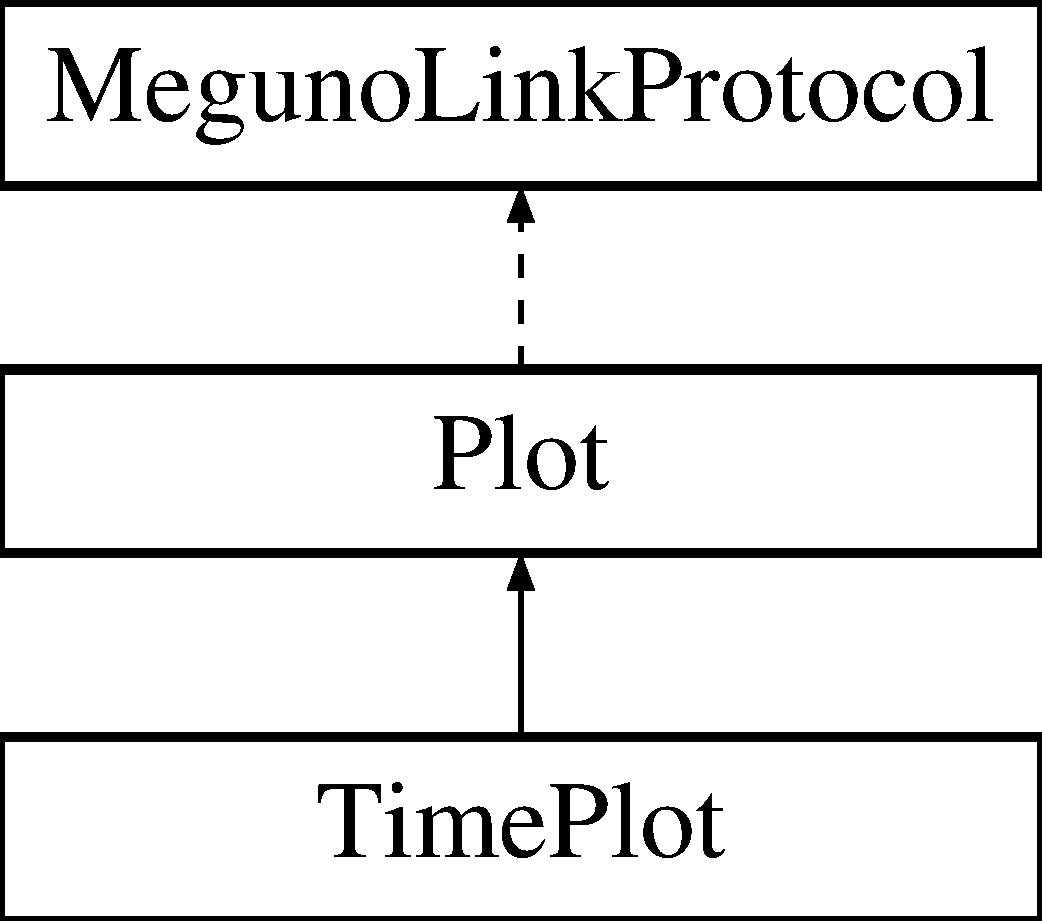
\includegraphics[height=3.000000cm]{class_time_plot}
\end{center}
\end{figure}
\subsection*{Public Member Functions}
\begin{DoxyCompactItemize}
\item 
\hyperlink{class_time_plot_a8d0140572be69a6270552b9180ff1e38}{Time\-Plot} (const char $\ast$channel\-Name=N\-U\-L\-L)
\item 
\hyperlink{class_time_plot_a2c5a3ade229494c3d0e285a7d3b55add}{Time\-Plot} (const \-\_\-\-\_\-\-Flash\-String\-Helper $\ast$channel\-Name)
\item 
{\footnotesize template$<$class T\-Y\-Data $>$ }\\void \hyperlink{class_time_plot_a15555221a62dc532d69211d639acf412}{Send\-Data} (const char $\ast$series\-Name, T\-Y\-Data y\-Value, const char $\ast$series\-Properties=N\-U\-L\-L)
\item 
{\footnotesize template$<$class T\-Y\-Data $>$ }\\void \hyperlink{class_time_plot_a72c411fcef4241143981dfe46b8bd0b8}{Send\-Data} (const char $\ast$series\-Name, T\-Y\-Data y\-Value, \hyperlink{class_plot_af4d6704578791a812f3f78617adc7040}{Colors} Color, \hyperlink{class_plot_a05a5ea232f5115847a9861a9660205c7}{Line\-Style} Line=\hyperlink{class_plot_a05a5ea232f5115847a9861a9660205c7a4a144f2b97cc3762d40863bde0853f22}{Solid}, uint8\-\_\-t u\-Line\-Width=1, \hyperlink{class_plot_a888bde9c76bb38843a5ab09097cbeeab}{Marker\-Style} Marker=\hyperlink{class_plot_a888bde9c76bb38843a5ab09097cbeeaba9eb079a6c0fcf4d7125147671b071e2e}{Circle})
\item 
void \hyperlink{class_time_plot_ac28dbd64c6900d80f9ef901d4391f46d}{Send\-Float\-Data} (const char $\ast$series\-Name, float y\-Value, int n\-Decimal\-Places, const char $\ast$series\-Properties=N\-U\-L\-L)
\item 
void \hyperlink{class_time_plot_a69f54f61224cd683732978d314206aec}{Send\-Float\-Data} (const char $\ast$series\-Name, float y\-Value, int n\-Decimal\-Places, \hyperlink{class_plot_af4d6704578791a812f3f78617adc7040}{Colors} Color, \hyperlink{class_plot_a05a5ea232f5115847a9861a9660205c7}{Line\-Style} Line=\hyperlink{class_plot_a05a5ea232f5115847a9861a9660205c7a4a144f2b97cc3762d40863bde0853f22}{Solid}, uint8\-\_\-t u\-Line\-Width=1, \hyperlink{class_plot_a888bde9c76bb38843a5ab09097cbeeab}{Marker\-Style} Marker=\hyperlink{class_plot_a888bde9c76bb38843a5ab09097cbeeaba9eb079a6c0fcf4d7125147671b071e2e}{Circle})
\item 
{\footnotesize template$<$class T\-Y\-Data $>$ }\\void \hyperlink{class_time_plot_a30570da83785d7d4ce8a38b4e6cc21de}{Send\-Data} (const \-\_\-\-\_\-\-Flash\-String\-Helper $\ast$series\-Name, T\-Y\-Data y\-Value, const char $\ast$series\-Properties=N\-U\-L\-L)
\item 
void \hyperlink{class_time_plot_a8b1f5f200af3ea81b6b481c7560839fc}{Send\-Float\-Data} (const \-\_\-\-\_\-\-Flash\-String\-Helper $\ast$series\-Name, float y\-Value, int n\-Decimal\-Places, const char $\ast$series\-Properties=N\-U\-L\-L)
\item 
void \hyperlink{class_time_plot_aa7944c43852b8029a409218554653b79}{Send\-Float\-Data} (const \-\_\-\-\_\-\-Flash\-String\-Helper $\ast$series\-Name, float y\-Value, int n\-Decimal\-Places, \hyperlink{class_plot_af4d6704578791a812f3f78617adc7040}{Colors} Color, \hyperlink{class_plot_a05a5ea232f5115847a9861a9660205c7}{Line\-Style} Line=\hyperlink{class_plot_a05a5ea232f5115847a9861a9660205c7a4a144f2b97cc3762d40863bde0853f22}{Solid}, uint8\-\_\-t u\-Line\-Width=1, \hyperlink{class_plot_a888bde9c76bb38843a5ab09097cbeeab}{Marker\-Style} Marker=\hyperlink{class_plot_a888bde9c76bb38843a5ab09097cbeeaba9eb079a6c0fcf4d7125147671b071e2e}{Circle})
\end{DoxyCompactItemize}
\subsection*{Additional Inherited Members}


\subsection{Constructor \& Destructor Documentation}
\hypertarget{class_time_plot_a8d0140572be69a6270552b9180ff1e38}{\index{Time\-Plot@{Time\-Plot}!Time\-Plot@{Time\-Plot}}
\index{Time\-Plot@{Time\-Plot}!TimePlot@{Time\-Plot}}
\subsubsection[{Time\-Plot}]{\setlength{\rightskip}{0pt plus 5cm}Time\-Plot\-::\-Time\-Plot (
\begin{DoxyParamCaption}
\item[{const char $\ast$}]{channel\-Name = {\ttfamily NULL}}
\end{DoxyParamCaption}
)}}\label{class_time_plot_a8d0140572be69a6270552b9180ff1e38}
\hypertarget{class_time_plot_a2c5a3ade229494c3d0e285a7d3b55add}{\index{Time\-Plot@{Time\-Plot}!Time\-Plot@{Time\-Plot}}
\index{Time\-Plot@{Time\-Plot}!TimePlot@{Time\-Plot}}
\subsubsection[{Time\-Plot}]{\setlength{\rightskip}{0pt plus 5cm}Time\-Plot\-::\-Time\-Plot (
\begin{DoxyParamCaption}
\item[{const \-\_\-\-\_\-\-Flash\-String\-Helper $\ast$}]{channel\-Name}
\end{DoxyParamCaption}
)}}\label{class_time_plot_a2c5a3ade229494c3d0e285a7d3b55add}


\subsection{Member Function Documentation}
\hypertarget{class_time_plot_a15555221a62dc532d69211d639acf412}{\index{Time\-Plot@{Time\-Plot}!Send\-Data@{Send\-Data}}
\index{Send\-Data@{Send\-Data}!TimePlot@{Time\-Plot}}
\subsubsection[{Send\-Data}]{\setlength{\rightskip}{0pt plus 5cm}template$<$class T\-Y\-Data $>$ void Time\-Plot\-::\-Send\-Data (
\begin{DoxyParamCaption}
\item[{const char $\ast$}]{series\-Name, }
\item[{T\-Y\-Data}]{y\-Value, }
\item[{const char $\ast$}]{series\-Properties = {\ttfamily NULL}}
\end{DoxyParamCaption}
)\hspace{0.3cm}{\ttfamily [inline]}}}\label{class_time_plot_a15555221a62dc532d69211d639acf412}
\hypertarget{class_time_plot_a72c411fcef4241143981dfe46b8bd0b8}{\index{Time\-Plot@{Time\-Plot}!Send\-Data@{Send\-Data}}
\index{Send\-Data@{Send\-Data}!TimePlot@{Time\-Plot}}
\subsubsection[{Send\-Data}]{\setlength{\rightskip}{0pt plus 5cm}template$<$class T\-Y\-Data $>$ void Time\-Plot\-::\-Send\-Data (
\begin{DoxyParamCaption}
\item[{const char $\ast$}]{series\-Name, }
\item[{T\-Y\-Data}]{y\-Value, }
\item[{{\bf Colors}}]{Color, }
\item[{{\bf Line\-Style}}]{Line = {\ttfamily {\bf Solid}}, }
\item[{uint8\-\_\-t}]{u\-Line\-Width = {\ttfamily 1}, }
\item[{{\bf Marker\-Style}}]{Marker = {\ttfamily {\bf Circle}}}
\end{DoxyParamCaption}
)\hspace{0.3cm}{\ttfamily [inline]}}}\label{class_time_plot_a72c411fcef4241143981dfe46b8bd0b8}
\hypertarget{class_time_plot_a30570da83785d7d4ce8a38b4e6cc21de}{\index{Time\-Plot@{Time\-Plot}!Send\-Data@{Send\-Data}}
\index{Send\-Data@{Send\-Data}!TimePlot@{Time\-Plot}}
\subsubsection[{Send\-Data}]{\setlength{\rightskip}{0pt plus 5cm}template$<$class T\-Y\-Data $>$ void Time\-Plot\-::\-Send\-Data (
\begin{DoxyParamCaption}
\item[{const \-\_\-\-\_\-\-Flash\-String\-Helper $\ast$}]{series\-Name, }
\item[{T\-Y\-Data}]{y\-Value, }
\item[{const char $\ast$}]{series\-Properties = {\ttfamily NULL}}
\end{DoxyParamCaption}
)\hspace{0.3cm}{\ttfamily [inline]}}}\label{class_time_plot_a30570da83785d7d4ce8a38b4e6cc21de}
\hypertarget{class_time_plot_ac28dbd64c6900d80f9ef901d4391f46d}{\index{Time\-Plot@{Time\-Plot}!Send\-Float\-Data@{Send\-Float\-Data}}
\index{Send\-Float\-Data@{Send\-Float\-Data}!TimePlot@{Time\-Plot}}
\subsubsection[{Send\-Float\-Data}]{\setlength{\rightskip}{0pt plus 5cm}void Time\-Plot\-::\-Send\-Float\-Data (
\begin{DoxyParamCaption}
\item[{const char $\ast$}]{series\-Name, }
\item[{float}]{y\-Value, }
\item[{int}]{n\-Decimal\-Places, }
\item[{const char $\ast$}]{series\-Properties = {\ttfamily NULL}}
\end{DoxyParamCaption}
)}}\label{class_time_plot_ac28dbd64c6900d80f9ef901d4391f46d}
\hypertarget{class_time_plot_a69f54f61224cd683732978d314206aec}{\index{Time\-Plot@{Time\-Plot}!Send\-Float\-Data@{Send\-Float\-Data}}
\index{Send\-Float\-Data@{Send\-Float\-Data}!TimePlot@{Time\-Plot}}
\subsubsection[{Send\-Float\-Data}]{\setlength{\rightskip}{0pt plus 5cm}void Time\-Plot\-::\-Send\-Float\-Data (
\begin{DoxyParamCaption}
\item[{const char $\ast$}]{series\-Name, }
\item[{float}]{y\-Value, }
\item[{int}]{n\-Decimal\-Places, }
\item[{{\bf Colors}}]{Color, }
\item[{{\bf Line\-Style}}]{Line = {\ttfamily {\bf Solid}}, }
\item[{uint8\-\_\-t}]{u\-Line\-Width = {\ttfamily 1}, }
\item[{{\bf Marker\-Style}}]{Marker = {\ttfamily {\bf Circle}}}
\end{DoxyParamCaption}
)}}\label{class_time_plot_a69f54f61224cd683732978d314206aec}
\hypertarget{class_time_plot_a8b1f5f200af3ea81b6b481c7560839fc}{\index{Time\-Plot@{Time\-Plot}!Send\-Float\-Data@{Send\-Float\-Data}}
\index{Send\-Float\-Data@{Send\-Float\-Data}!TimePlot@{Time\-Plot}}
\subsubsection[{Send\-Float\-Data}]{\setlength{\rightskip}{0pt plus 5cm}void Time\-Plot\-::\-Send\-Float\-Data (
\begin{DoxyParamCaption}
\item[{const \-\_\-\-\_\-\-Flash\-String\-Helper $\ast$}]{series\-Name, }
\item[{float}]{y\-Value, }
\item[{int}]{n\-Decimal\-Places, }
\item[{const char $\ast$}]{series\-Properties = {\ttfamily NULL}}
\end{DoxyParamCaption}
)}}\label{class_time_plot_a8b1f5f200af3ea81b6b481c7560839fc}
\hypertarget{class_time_plot_aa7944c43852b8029a409218554653b79}{\index{Time\-Plot@{Time\-Plot}!Send\-Float\-Data@{Send\-Float\-Data}}
\index{Send\-Float\-Data@{Send\-Float\-Data}!TimePlot@{Time\-Plot}}
\subsubsection[{Send\-Float\-Data}]{\setlength{\rightskip}{0pt plus 5cm}void Time\-Plot\-::\-Send\-Float\-Data (
\begin{DoxyParamCaption}
\item[{const \-\_\-\-\_\-\-Flash\-String\-Helper $\ast$}]{series\-Name, }
\item[{float}]{y\-Value, }
\item[{int}]{n\-Decimal\-Places, }
\item[{{\bf Colors}}]{Color, }
\item[{{\bf Line\-Style}}]{Line = {\ttfamily {\bf Solid}}, }
\item[{uint8\-\_\-t}]{u\-Line\-Width = {\ttfamily 1}, }
\item[{{\bf Marker\-Style}}]{Marker = {\ttfamily {\bf Circle}}}
\end{DoxyParamCaption}
)}}\label{class_time_plot_aa7944c43852b8029a409218554653b79}


The documentation for this class was generated from the following files\-:\begin{DoxyCompactItemize}
\item 
/\-Dropbox/\-Arduino\-Development/\-Git\-Hub/\-M\-L\-P/utility/\hyperlink{_time_plot_8h}{Time\-Plot.\-h}\item 
/\-Dropbox/\-Arduino\-Development/\-Git\-Hub/\-M\-L\-P/utility/\hyperlink{_time_plot_8cpp}{Time\-Plot.\-cpp}\end{DoxyCompactItemize}

\hypertarget{class_x_y_plot}{\section{X\-Y\-Plot Class Reference}
\label{class_x_y_plot}\index{X\-Y\-Plot@{X\-Y\-Plot}}
}


{\ttfamily \#include $<$X\-Y\-Plot.\-h$>$}

Inheritance diagram for X\-Y\-Plot\-:\begin{figure}[H]
\begin{center}
\leavevmode
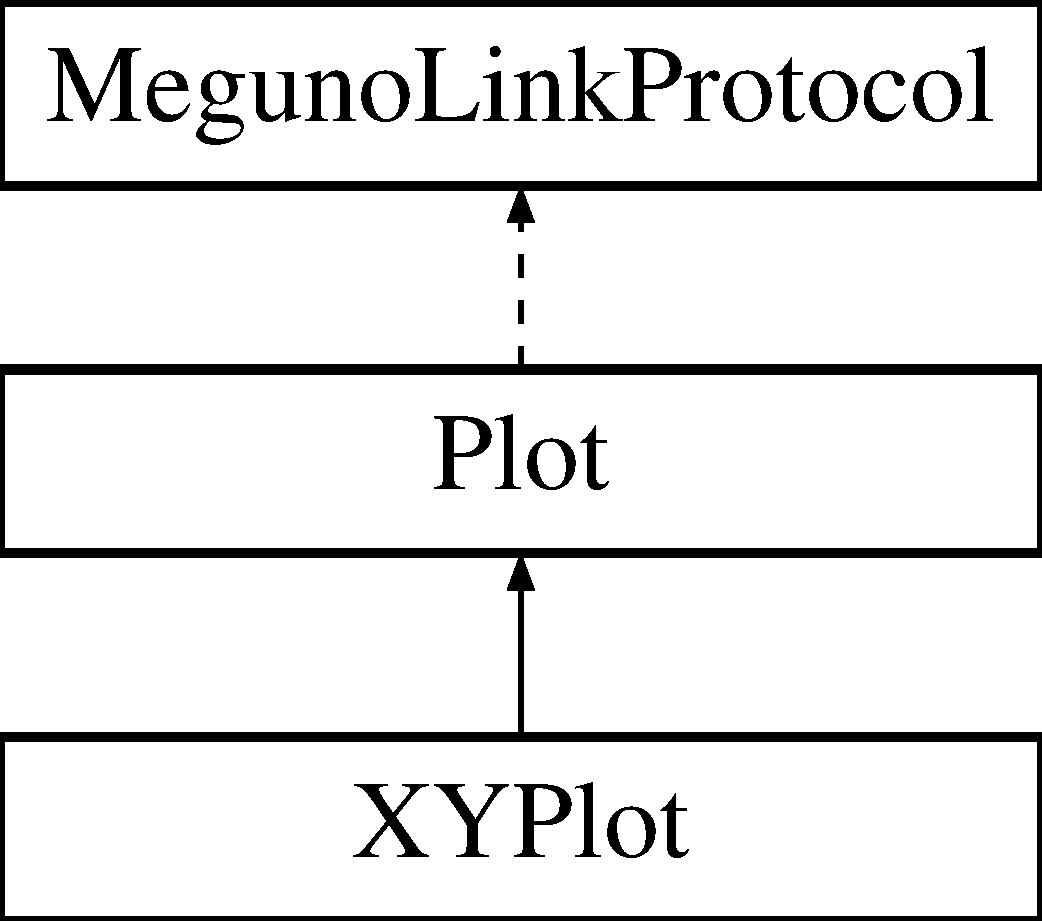
\includegraphics[height=3.000000cm]{class_x_y_plot}
\end{center}
\end{figure}
\subsection*{Public Member Functions}
\begin{DoxyCompactItemize}
\item 
\hyperlink{class_x_y_plot_a2eb15ab7b978250fadb0c17641f3d559}{X\-Y\-Plot} (const char $\ast$channel\-Name=N\-U\-L\-L)
\item 
\hyperlink{class_x_y_plot_ac1da6343667a85e50927e6a7c0f8e8e0}{X\-Y\-Plot} (const \-\_\-\-\_\-\-Flash\-String\-Helper $\ast$channel\-Name)
\item 
{\footnotesize template$<$class T\-X\-Data , class T\-Y\-Data $>$ }\\void \hyperlink{class_x_y_plot_ad224fe41ae8cd8f1c226c826e577e9f7}{Send\-Data} (const char $\ast$series\-Name, T\-X\-Data x\-Value, T\-Y\-Data y\-Value, const char $\ast$series\-Properties=N\-U\-L\-L)
\item 
{\footnotesize template$<$class T\-X\-Data , class T\-Y\-Data $>$ }\\void \hyperlink{class_x_y_plot_aea1795e7bc4d61a10427c7a251f926b6}{Send\-Data} (const char $\ast$series\-Name, T\-X\-Data x\-Value, T\-Y\-Data y\-Value, \hyperlink{class_plot_af4d6704578791a812f3f78617adc7040}{Colors} Color, \hyperlink{class_plot_a05a5ea232f5115847a9861a9660205c7}{Line\-Style} Line=\hyperlink{class_plot_a05a5ea232f5115847a9861a9660205c7a4a144f2b97cc3762d40863bde0853f22}{Solid}, uint8\-\_\-t u\-Line\-Width=1, \hyperlink{class_plot_a888bde9c76bb38843a5ab09097cbeeab}{Marker\-Style} Marker=\hyperlink{class_plot_a888bde9c76bb38843a5ab09097cbeeaba9eb079a6c0fcf4d7125147671b071e2e}{Circle})
\item 
{\footnotesize template$<$class T\-X\-Data $>$ }\\void \hyperlink{class_x_y_plot_a7a7ae0fce5ebee29cb11fd5b858ed012}{Send\-Data} (const char $\ast$series\-Name, T\-X\-Data x\-Value, float y\-Value, int n\-Decimal\-Places, const char $\ast$series\-Properties=N\-U\-L\-L)
\item 
{\footnotesize template$<$class T\-X\-Data $>$ }\\void \hyperlink{class_x_y_plot_ab779ba9752cc633b55ea68b23d29d27f}{Send\-Data} (const char $\ast$series\-Name, T\-X\-Data x\-Value, float y\-Value, int n\-Decimal\-Places, \hyperlink{class_plot_af4d6704578791a812f3f78617adc7040}{Colors} Color, \hyperlink{class_plot_a05a5ea232f5115847a9861a9660205c7}{Line\-Style} Line=\hyperlink{class_plot_a05a5ea232f5115847a9861a9660205c7a4a144f2b97cc3762d40863bde0853f22}{Solid}, uint8\-\_\-t u\-Line\-Width=1, \hyperlink{class_plot_a888bde9c76bb38843a5ab09097cbeeab}{Marker\-Style} Marker=\hyperlink{class_plot_a888bde9c76bb38843a5ab09097cbeeaba9eb079a6c0fcf4d7125147671b071e2e}{Circle})
\item 
{\footnotesize template$<$class T\-X\-Data , class T\-Y\-Data $>$ }\\void \hyperlink{class_x_y_plot_ad6f8fbd31b4b94aaf47bacf2526d7737}{Send\-Data} (const \-\_\-\-\_\-\-Flash\-String\-Helper $\ast$series\-Name, T\-X\-Data x\-Value, T\-Y\-Data y\-Value, const char $\ast$series\-Properties=N\-U\-L\-L)
\item 
{\footnotesize template$<$class T\-X\-Data , class T\-Y\-Data $>$ }\\void \hyperlink{class_x_y_plot_afe1bf4cbb0c50ef5e12d327679111546}{Send\-Data} (const \-\_\-\-\_\-\-Flash\-String\-Helper $\ast$series\-Name, T\-X\-Data x\-Value, T\-Y\-Data y\-Value, \hyperlink{class_plot_af4d6704578791a812f3f78617adc7040}{Colors} Color, \hyperlink{class_plot_a05a5ea232f5115847a9861a9660205c7}{Line\-Style} Line=\hyperlink{class_plot_a05a5ea232f5115847a9861a9660205c7a4a144f2b97cc3762d40863bde0853f22}{Solid}, uint8\-\_\-t u\-Line\-Width=1, \hyperlink{class_plot_a888bde9c76bb38843a5ab09097cbeeab}{Marker\-Style} Marker=\hyperlink{class_plot_a888bde9c76bb38843a5ab09097cbeeaba9eb079a6c0fcf4d7125147671b071e2e}{Circle})
\item 
{\footnotesize template$<$class T\-X\-Data $>$ }\\void \hyperlink{class_x_y_plot_adb75abc61f0cfe383f224bd1f5bf3f22}{Send\-Data} (const \-\_\-\-\_\-\-Flash\-String\-Helper $\ast$series\-Name, T\-X\-Data x\-Value, float y\-Value, int n\-Decimal\-Places, const char $\ast$series\-Properties=N\-U\-L\-L)
\item 
{\footnotesize template$<$class T\-X\-Data $>$ }\\void \hyperlink{class_x_y_plot_ab31b7d4dd77799d25c79f1461d3826fb}{Send\-Data} (const \-\_\-\-\_\-\-Flash\-String\-Helper $\ast$series\-Name, T\-X\-Data x\-Value, float y\-Value, int n\-Decimal\-Places, \hyperlink{class_plot_af4d6704578791a812f3f78617adc7040}{Colors} Color, \hyperlink{class_plot_a05a5ea232f5115847a9861a9660205c7}{Line\-Style} Line=\hyperlink{class_plot_a05a5ea232f5115847a9861a9660205c7a4a144f2b97cc3762d40863bde0853f22}{Solid}, uint8\-\_\-t u\-Line\-Width=1, \hyperlink{class_plot_a888bde9c76bb38843a5ab09097cbeeab}{Marker\-Style} Marker=\hyperlink{class_plot_a888bde9c76bb38843a5ab09097cbeeaba9eb079a6c0fcf4d7125147671b071e2e}{Circle})
\end{DoxyCompactItemize}
\subsection*{Additional Inherited Members}


\subsection{Constructor \& Destructor Documentation}
\hypertarget{class_x_y_plot_a2eb15ab7b978250fadb0c17641f3d559}{\index{X\-Y\-Plot@{X\-Y\-Plot}!X\-Y\-Plot@{X\-Y\-Plot}}
\index{X\-Y\-Plot@{X\-Y\-Plot}!XYPlot@{X\-Y\-Plot}}
\subsubsection[{X\-Y\-Plot}]{\setlength{\rightskip}{0pt plus 5cm}X\-Y\-Plot\-::\-X\-Y\-Plot (
\begin{DoxyParamCaption}
\item[{const char $\ast$}]{channel\-Name = {\ttfamily NULL}}
\end{DoxyParamCaption}
)}}\label{class_x_y_plot_a2eb15ab7b978250fadb0c17641f3d559}
\hypertarget{class_x_y_plot_ac1da6343667a85e50927e6a7c0f8e8e0}{\index{X\-Y\-Plot@{X\-Y\-Plot}!X\-Y\-Plot@{X\-Y\-Plot}}
\index{X\-Y\-Plot@{X\-Y\-Plot}!XYPlot@{X\-Y\-Plot}}
\subsubsection[{X\-Y\-Plot}]{\setlength{\rightskip}{0pt plus 5cm}X\-Y\-Plot\-::\-X\-Y\-Plot (
\begin{DoxyParamCaption}
\item[{const \-\_\-\-\_\-\-Flash\-String\-Helper $\ast$}]{channel\-Name}
\end{DoxyParamCaption}
)}}\label{class_x_y_plot_ac1da6343667a85e50927e6a7c0f8e8e0}


\subsection{Member Function Documentation}
\hypertarget{class_x_y_plot_ad224fe41ae8cd8f1c226c826e577e9f7}{\index{X\-Y\-Plot@{X\-Y\-Plot}!Send\-Data@{Send\-Data}}
\index{Send\-Data@{Send\-Data}!XYPlot@{X\-Y\-Plot}}
\subsubsection[{Send\-Data}]{\setlength{\rightskip}{0pt plus 5cm}template$<$class T\-X\-Data , class T\-Y\-Data $>$ void X\-Y\-Plot\-::\-Send\-Data (
\begin{DoxyParamCaption}
\item[{const char $\ast$}]{series\-Name, }
\item[{T\-X\-Data}]{x\-Value, }
\item[{T\-Y\-Data}]{y\-Value, }
\item[{const char $\ast$}]{series\-Properties = {\ttfamily NULL}}
\end{DoxyParamCaption}
)\hspace{0.3cm}{\ttfamily [inline]}}}\label{class_x_y_plot_ad224fe41ae8cd8f1c226c826e577e9f7}
\hypertarget{class_x_y_plot_aea1795e7bc4d61a10427c7a251f926b6}{\index{X\-Y\-Plot@{X\-Y\-Plot}!Send\-Data@{Send\-Data}}
\index{Send\-Data@{Send\-Data}!XYPlot@{X\-Y\-Plot}}
\subsubsection[{Send\-Data}]{\setlength{\rightskip}{0pt plus 5cm}template$<$class T\-X\-Data , class T\-Y\-Data $>$ void X\-Y\-Plot\-::\-Send\-Data (
\begin{DoxyParamCaption}
\item[{const char $\ast$}]{series\-Name, }
\item[{T\-X\-Data}]{x\-Value, }
\item[{T\-Y\-Data}]{y\-Value, }
\item[{{\bf Colors}}]{Color, }
\item[{{\bf Line\-Style}}]{Line = {\ttfamily {\bf Solid}}, }
\item[{uint8\-\_\-t}]{u\-Line\-Width = {\ttfamily 1}, }
\item[{{\bf Marker\-Style}}]{Marker = {\ttfamily {\bf Circle}}}
\end{DoxyParamCaption}
)\hspace{0.3cm}{\ttfamily [inline]}}}\label{class_x_y_plot_aea1795e7bc4d61a10427c7a251f926b6}
\hypertarget{class_x_y_plot_a7a7ae0fce5ebee29cb11fd5b858ed012}{\index{X\-Y\-Plot@{X\-Y\-Plot}!Send\-Data@{Send\-Data}}
\index{Send\-Data@{Send\-Data}!XYPlot@{X\-Y\-Plot}}
\subsubsection[{Send\-Data}]{\setlength{\rightskip}{0pt plus 5cm}template$<$class T\-X\-Data $>$ void X\-Y\-Plot\-::\-Send\-Data (
\begin{DoxyParamCaption}
\item[{const char $\ast$}]{series\-Name, }
\item[{T\-X\-Data}]{x\-Value, }
\item[{float}]{y\-Value, }
\item[{int}]{n\-Decimal\-Places, }
\item[{const char $\ast$}]{series\-Properties = {\ttfamily NULL}}
\end{DoxyParamCaption}
)\hspace{0.3cm}{\ttfamily [inline]}}}\label{class_x_y_plot_a7a7ae0fce5ebee29cb11fd5b858ed012}
\hypertarget{class_x_y_plot_ab779ba9752cc633b55ea68b23d29d27f}{\index{X\-Y\-Plot@{X\-Y\-Plot}!Send\-Data@{Send\-Data}}
\index{Send\-Data@{Send\-Data}!XYPlot@{X\-Y\-Plot}}
\subsubsection[{Send\-Data}]{\setlength{\rightskip}{0pt plus 5cm}template$<$class T\-X\-Data $>$ void X\-Y\-Plot\-::\-Send\-Data (
\begin{DoxyParamCaption}
\item[{const char $\ast$}]{series\-Name, }
\item[{T\-X\-Data}]{x\-Value, }
\item[{float}]{y\-Value, }
\item[{int}]{n\-Decimal\-Places, }
\item[{{\bf Colors}}]{Color, }
\item[{{\bf Line\-Style}}]{Line = {\ttfamily {\bf Solid}}, }
\item[{uint8\-\_\-t}]{u\-Line\-Width = {\ttfamily 1}, }
\item[{{\bf Marker\-Style}}]{Marker = {\ttfamily {\bf Circle}}}
\end{DoxyParamCaption}
)\hspace{0.3cm}{\ttfamily [inline]}}}\label{class_x_y_plot_ab779ba9752cc633b55ea68b23d29d27f}
\hypertarget{class_x_y_plot_ad6f8fbd31b4b94aaf47bacf2526d7737}{\index{X\-Y\-Plot@{X\-Y\-Plot}!Send\-Data@{Send\-Data}}
\index{Send\-Data@{Send\-Data}!XYPlot@{X\-Y\-Plot}}
\subsubsection[{Send\-Data}]{\setlength{\rightskip}{0pt plus 5cm}template$<$class T\-X\-Data , class T\-Y\-Data $>$ void X\-Y\-Plot\-::\-Send\-Data (
\begin{DoxyParamCaption}
\item[{const \-\_\-\-\_\-\-Flash\-String\-Helper $\ast$}]{series\-Name, }
\item[{T\-X\-Data}]{x\-Value, }
\item[{T\-Y\-Data}]{y\-Value, }
\item[{const char $\ast$}]{series\-Properties = {\ttfamily NULL}}
\end{DoxyParamCaption}
)\hspace{0.3cm}{\ttfamily [inline]}}}\label{class_x_y_plot_ad6f8fbd31b4b94aaf47bacf2526d7737}
\hypertarget{class_x_y_plot_afe1bf4cbb0c50ef5e12d327679111546}{\index{X\-Y\-Plot@{X\-Y\-Plot}!Send\-Data@{Send\-Data}}
\index{Send\-Data@{Send\-Data}!XYPlot@{X\-Y\-Plot}}
\subsubsection[{Send\-Data}]{\setlength{\rightskip}{0pt plus 5cm}template$<$class T\-X\-Data , class T\-Y\-Data $>$ void X\-Y\-Plot\-::\-Send\-Data (
\begin{DoxyParamCaption}
\item[{const \-\_\-\-\_\-\-Flash\-String\-Helper $\ast$}]{series\-Name, }
\item[{T\-X\-Data}]{x\-Value, }
\item[{T\-Y\-Data}]{y\-Value, }
\item[{{\bf Colors}}]{Color, }
\item[{{\bf Line\-Style}}]{Line = {\ttfamily {\bf Solid}}, }
\item[{uint8\-\_\-t}]{u\-Line\-Width = {\ttfamily 1}, }
\item[{{\bf Marker\-Style}}]{Marker = {\ttfamily {\bf Circle}}}
\end{DoxyParamCaption}
)\hspace{0.3cm}{\ttfamily [inline]}}}\label{class_x_y_plot_afe1bf4cbb0c50ef5e12d327679111546}
\hypertarget{class_x_y_plot_adb75abc61f0cfe383f224bd1f5bf3f22}{\index{X\-Y\-Plot@{X\-Y\-Plot}!Send\-Data@{Send\-Data}}
\index{Send\-Data@{Send\-Data}!XYPlot@{X\-Y\-Plot}}
\subsubsection[{Send\-Data}]{\setlength{\rightskip}{0pt plus 5cm}template$<$class T\-X\-Data $>$ void X\-Y\-Plot\-::\-Send\-Data (
\begin{DoxyParamCaption}
\item[{const \-\_\-\-\_\-\-Flash\-String\-Helper $\ast$}]{series\-Name, }
\item[{T\-X\-Data}]{x\-Value, }
\item[{float}]{y\-Value, }
\item[{int}]{n\-Decimal\-Places, }
\item[{const char $\ast$}]{series\-Properties = {\ttfamily NULL}}
\end{DoxyParamCaption}
)\hspace{0.3cm}{\ttfamily [inline]}}}\label{class_x_y_plot_adb75abc61f0cfe383f224bd1f5bf3f22}
\hypertarget{class_x_y_plot_ab31b7d4dd77799d25c79f1461d3826fb}{\index{X\-Y\-Plot@{X\-Y\-Plot}!Send\-Data@{Send\-Data}}
\index{Send\-Data@{Send\-Data}!XYPlot@{X\-Y\-Plot}}
\subsubsection[{Send\-Data}]{\setlength{\rightskip}{0pt plus 5cm}template$<$class T\-X\-Data $>$ void X\-Y\-Plot\-::\-Send\-Data (
\begin{DoxyParamCaption}
\item[{const \-\_\-\-\_\-\-Flash\-String\-Helper $\ast$}]{series\-Name, }
\item[{T\-X\-Data}]{x\-Value, }
\item[{float}]{y\-Value, }
\item[{int}]{n\-Decimal\-Places, }
\item[{{\bf Colors}}]{Color, }
\item[{{\bf Line\-Style}}]{Line = {\ttfamily {\bf Solid}}, }
\item[{uint8\-\_\-t}]{u\-Line\-Width = {\ttfamily 1}, }
\item[{{\bf Marker\-Style}}]{Marker = {\ttfamily {\bf Circle}}}
\end{DoxyParamCaption}
)\hspace{0.3cm}{\ttfamily [inline]}}}\label{class_x_y_plot_ab31b7d4dd77799d25c79f1461d3826fb}


The documentation for this class was generated from the following files\-:\begin{DoxyCompactItemize}
\item 
/\-Dropbox/\-Arduino\-Development/\-Git\-Hub/\-M\-L\-P/utility/\hyperlink{_x_y_plot_8h}{X\-Y\-Plot.\-h}\item 
/\-Dropbox/\-Arduino\-Development/\-Git\-Hub/\-M\-L\-P/utility/\hyperlink{_x_y_plot_8cpp}{X\-Y\-Plot.\-cpp}\end{DoxyCompactItemize}

\chapter{File Documentation}
\hypertarget{_meguno_link_8h}{\section{/\-Dropbox/\-Arduino\-Development/\-Git\-Hub/\-M\-L\-P/\-Meguno\-Link.h File Reference}
\label{_meguno_link_8h}\index{/\-Dropbox/\-Arduino\-Development/\-Git\-Hub/\-M\-L\-P/\-Meguno\-Link.\-h@{/\-Dropbox/\-Arduino\-Development/\-Git\-Hub/\-M\-L\-P/\-Meguno\-Link.\-h}}
}
{\ttfamily \#include \char`\"{}utility\textbackslash{}\-Interface\-Panel.\-h\char`\"{}}\\*
{\ttfamily \#include \char`\"{}utility\textbackslash{}\-Map.\-h\char`\"{}}\\*
{\ttfamily \#include \char`\"{}utility\textbackslash{}\-Message.\-h\char`\"{}}\\*
{\ttfamily \#include \char`\"{}utility\textbackslash{}\-Table.\-h\char`\"{}}\\*
{\ttfamily \#include \char`\"{}utility\textbackslash{}\-Time\-Plot.\-h\char`\"{}}\\*
{\ttfamily \#include \char`\"{}utility\textbackslash{}\-X\-Y\-Plot.\-h\char`\"{}}\\*

\hypertarget{_r_e_a_d_m_e_8md}{\section{/\-Dropbox/\-Arduino\-Development/\-Git\-Hub/\-M\-L\-P/\-R\-E\-A\-D\-M\-E.md File Reference}
\label{_r_e_a_d_m_e_8md}\index{/\-Dropbox/\-Arduino\-Development/\-Git\-Hub/\-M\-L\-P/\-R\-E\-A\-D\-M\-E.\-md@{/\-Dropbox/\-Arduino\-Development/\-Git\-Hub/\-M\-L\-P/\-R\-E\-A\-D\-M\-E.\-md}}
}

\hypertarget{_interface_panel_8cpp}{\section{/\-Dropbox/\-Arduino\-Development/\-Git\-Hub/\-M\-L\-P/utility/\-Interface\-Panel.cpp File Reference}
\label{_interface_panel_8cpp}\index{/\-Dropbox/\-Arduino\-Development/\-Git\-Hub/\-M\-L\-P/utility/\-Interface\-Panel.\-cpp@{/\-Dropbox/\-Arduino\-Development/\-Git\-Hub/\-M\-L\-P/utility/\-Interface\-Panel.\-cpp}}
}
{\ttfamily \#include \char`\"{}Interface\-Panel.\-h\char`\"{}}\\*

\hypertarget{_interface_panel_8h}{\section{/\-Dropbox/\-Arduino\-Development/\-Git\-Hub/\-M\-L\-P/utility/\-Interface\-Panel.h File Reference}
\label{_interface_panel_8h}\index{/\-Dropbox/\-Arduino\-Development/\-Git\-Hub/\-M\-L\-P/utility/\-Interface\-Panel.\-h@{/\-Dropbox/\-Arduino\-Development/\-Git\-Hub/\-M\-L\-P/utility/\-Interface\-Panel.\-h}}
}
{\ttfamily \#include $<$Arduino.\-h$>$}\\*
{\ttfamily \#include \char`\"{}Meguno\-Link\-Protocol.\-h\char`\"{}}\\*
\subsection*{Classes}
\begin{DoxyCompactItemize}
\item 
class \hyperlink{class_interface_panel}{Interface\-Panel}
\end{DoxyCompactItemize}

\hypertarget{_map_8cpp}{\section{/\-Dropbox/\-Arduino\-Development/\-Git\-Hub/\-M\-L\-P/utility/\-Map.cpp File Reference}
\label{_map_8cpp}\index{/\-Dropbox/\-Arduino\-Development/\-Git\-Hub/\-M\-L\-P/utility/\-Map.\-cpp@{/\-Dropbox/\-Arduino\-Development/\-Git\-Hub/\-M\-L\-P/utility/\-Map.\-cpp}}
}
{\ttfamily \#include \char`\"{}Map.\-h\char`\"{}}\\*

\hypertarget{_map_8h}{\section{/\-Dropbox/\-Arduino\-Development/\-Git\-Hub/\-M\-L\-P/utility/\-Map.h File Reference}
\label{_map_8h}\index{/\-Dropbox/\-Arduino\-Development/\-Git\-Hub/\-M\-L\-P/utility/\-Map.\-h@{/\-Dropbox/\-Arduino\-Development/\-Git\-Hub/\-M\-L\-P/utility/\-Map.\-h}}
}
{\ttfamily \#include \char`\"{}Meguno\-Link\-Protocol.\-h\char`\"{}}\\*
\subsection*{Classes}
\begin{DoxyCompactItemize}
\item 
class \hyperlink{class_map}{Map}
\end{DoxyCompactItemize}

\hypertarget{_meguno_link_protocol_8cpp}{\section{/\-Dropbox/\-Arduino\-Development/\-Git\-Hub/\-M\-L\-P/utility/\-Meguno\-Link\-Protocol.cpp File Reference}
\label{_meguno_link_protocol_8cpp}\index{/\-Dropbox/\-Arduino\-Development/\-Git\-Hub/\-M\-L\-P/utility/\-Meguno\-Link\-Protocol.\-cpp@{/\-Dropbox/\-Arduino\-Development/\-Git\-Hub/\-M\-L\-P/utility/\-Meguno\-Link\-Protocol.\-cpp}}
}
{\ttfamily \#include \char`\"{}Meguno\-Link\-Protocol.\-h\char`\"{}}\\*

\hypertarget{_meguno_link_protocol_8h}{\section{/\-Dropbox/\-Arduino\-Development/\-Git\-Hub/\-M\-L\-P/utility/\-Meguno\-Link\-Protocol.h File Reference}
\label{_meguno_link_protocol_8h}\index{/\-Dropbox/\-Arduino\-Development/\-Git\-Hub/\-M\-L\-P/utility/\-Meguno\-Link\-Protocol.\-h@{/\-Dropbox/\-Arduino\-Development/\-Git\-Hub/\-M\-L\-P/utility/\-Meguno\-Link\-Protocol.\-h}}
}
{\ttfamily \#include $<$Arduino.\-h$>$}\\*
\subsection*{Classes}
\begin{DoxyCompactItemize}
\item 
class \hyperlink{class_meguno_link_protocol}{Meguno\-Link\-Protocol}
\end{DoxyCompactItemize}

\hypertarget{_message_8cpp}{\section{/\-Dropbox/\-Arduino\-Development/\-Git\-Hub/\-M\-L\-P/utility/\-Message.cpp File Reference}
\label{_message_8cpp}\index{/\-Dropbox/\-Arduino\-Development/\-Git\-Hub/\-M\-L\-P/utility/\-Message.\-cpp@{/\-Dropbox/\-Arduino\-Development/\-Git\-Hub/\-M\-L\-P/utility/\-Message.\-cpp}}
}
{\ttfamily \#include \char`\"{}message.\-h\char`\"{}}\\*

\hypertarget{_message_8h}{\section{/\-Dropbox/\-Arduino\-Development/\-Git\-Hub/\-M\-L\-P/utility/\-Message.h File Reference}
\label{_message_8h}\index{/\-Dropbox/\-Arduino\-Development/\-Git\-Hub/\-M\-L\-P/utility/\-Message.\-h@{/\-Dropbox/\-Arduino\-Development/\-Git\-Hub/\-M\-L\-P/utility/\-Message.\-h}}
}
{\ttfamily \#include \char`\"{}Meguno\-Link\-Protocol.\-h\char`\"{}}\\*
\subsection*{Classes}
\begin{DoxyCompactItemize}
\item 
class \hyperlink{class_message}{Message}
\end{DoxyCompactItemize}

\hypertarget{_plot_8cpp}{\section{/\-Dropbox/\-Arduino\-Development/\-Git\-Hub/\-M\-L\-P/utility/\-Plot.cpp File Reference}
\label{_plot_8cpp}\index{/\-Dropbox/\-Arduino\-Development/\-Git\-Hub/\-M\-L\-P/utility/\-Plot.\-cpp@{/\-Dropbox/\-Arduino\-Development/\-Git\-Hub/\-M\-L\-P/utility/\-Plot.\-cpp}}
}
{\ttfamily \#include \char`\"{}Plot.\-h\char`\"{}}\\*

\hypertarget{_plot_8h}{\section{/\-Dropbox/\-Arduino\-Development/\-Git\-Hub/\-M\-L\-P/utility/\-Plot.h File Reference}
\label{_plot_8h}\index{/\-Dropbox/\-Arduino\-Development/\-Git\-Hub/\-M\-L\-P/utility/\-Plot.\-h@{/\-Dropbox/\-Arduino\-Development/\-Git\-Hub/\-M\-L\-P/utility/\-Plot.\-h}}
}
{\ttfamily \#include \char`\"{}Meguno\-Link\-Protocol.\-h\char`\"{}}\\*
\subsection*{Classes}
\begin{DoxyCompactItemize}
\item 
class \hyperlink{class_plot}{Plot}
\end{DoxyCompactItemize}

\hypertarget{_table_8cpp}{\section{/\-Dropbox/\-Arduino\-Development/\-Git\-Hub/\-M\-L\-P/utility/\-Table.cpp File Reference}
\label{_table_8cpp}\index{/\-Dropbox/\-Arduino\-Development/\-Git\-Hub/\-M\-L\-P/utility/\-Table.\-cpp@{/\-Dropbox/\-Arduino\-Development/\-Git\-Hub/\-M\-L\-P/utility/\-Table.\-cpp}}
}
{\ttfamily \#include \char`\"{}table.\-h\char`\"{}}\\*

\hypertarget{_table_8h}{\section{/\-Dropbox/\-Arduino\-Development/\-Git\-Hub/\-M\-L\-P/utility/\-Table.h File Reference}
\label{_table_8h}\index{/\-Dropbox/\-Arduino\-Development/\-Git\-Hub/\-M\-L\-P/utility/\-Table.\-h@{/\-Dropbox/\-Arduino\-Development/\-Git\-Hub/\-M\-L\-P/utility/\-Table.\-h}}
}
{\ttfamily \#include \char`\"{}Meguno\-Link\-Protocol.\-h\char`\"{}}\\*
\subsection*{Classes}
\begin{DoxyCompactItemize}
\item 
class \hyperlink{class_table}{Table}
\end{DoxyCompactItemize}

\hypertarget{_time_plot_8cpp}{\section{/\-Dropbox/\-Arduino\-Development/\-Git\-Hub/\-M\-L\-P/utility/\-Time\-Plot.cpp File Reference}
\label{_time_plot_8cpp}\index{/\-Dropbox/\-Arduino\-Development/\-Git\-Hub/\-M\-L\-P/utility/\-Time\-Plot.\-cpp@{/\-Dropbox/\-Arduino\-Development/\-Git\-Hub/\-M\-L\-P/utility/\-Time\-Plot.\-cpp}}
}
{\ttfamily \#include \char`\"{}Time\-Plot.\-h\char`\"{}}\\*

\hypertarget{_time_plot_8h}{\section{/\-Dropbox/\-Arduino\-Development/\-Git\-Hub/\-M\-L\-P/utility/\-Time\-Plot.h File Reference}
\label{_time_plot_8h}\index{/\-Dropbox/\-Arduino\-Development/\-Git\-Hub/\-M\-L\-P/utility/\-Time\-Plot.\-h@{/\-Dropbox/\-Arduino\-Development/\-Git\-Hub/\-M\-L\-P/utility/\-Time\-Plot.\-h}}
}
{\ttfamily \#include $<$Arduino.\-h$>$}\\*
{\ttfamily \#include \char`\"{}Plot.\-h\char`\"{}}\\*
\subsection*{Classes}
\begin{DoxyCompactItemize}
\item 
class \hyperlink{class_time_plot}{Time\-Plot}
\end{DoxyCompactItemize}

\hypertarget{_x_y_plot_8cpp}{\section{/\-Dropbox/\-Arduino\-Development/\-Git\-Hub/\-M\-L\-P/utility/\-X\-Y\-Plot.cpp File Reference}
\label{_x_y_plot_8cpp}\index{/\-Dropbox/\-Arduino\-Development/\-Git\-Hub/\-M\-L\-P/utility/\-X\-Y\-Plot.\-cpp@{/\-Dropbox/\-Arduino\-Development/\-Git\-Hub/\-M\-L\-P/utility/\-X\-Y\-Plot.\-cpp}}
}
{\ttfamily \#include \char`\"{}xyplot.\-h\char`\"{}}\\*

\hypertarget{_x_y_plot_8h}{\section{/\-Dropbox/\-Arduino\-Development/\-Git\-Hub/\-M\-L\-P/utility/\-X\-Y\-Plot.h File Reference}
\label{_x_y_plot_8h}\index{/\-Dropbox/\-Arduino\-Development/\-Git\-Hub/\-M\-L\-P/utility/\-X\-Y\-Plot.\-h@{/\-Dropbox/\-Arduino\-Development/\-Git\-Hub/\-M\-L\-P/utility/\-X\-Y\-Plot.\-h}}
}
{\ttfamily \#include $<$Arduino.\-h$>$}\\*
{\ttfamily \#include \char`\"{}Plot.\-h\char`\"{}}\\*
\subsection*{Classes}
\begin{DoxyCompactItemize}
\item 
class \hyperlink{class_x_y_plot}{X\-Y\-Plot}
\end{DoxyCompactItemize}

%--- End generated contents ---

% Index
\newpage
\phantomsection
\addcontentsline{toc}{chapter}{Index}
\printindex

\end{document}
